\documentclass[titlepage]{article}
\usepackage{luatextra}
\usepackage{polyglossia}
\usepackage{ulem}
\usepackage{framed}
\usepackage{color}
\usepackage{geometry}
\usepackage{amsmath}
\usepackage{unicode-math}
\usepackage[hidelinks]{hyperref}
\usepackage{latexsym}
\usepackage{pdflscape}
\usepackage{pdfpages}
\usepackage{enumitem}
\usepackage{titlesec}
\usepackage{lastpage}
\usepackage{fancyhdr}
\usepackage{titlesec}
\usepackage{listings}
\usepackage{graphicx}
\usepackage{float}
\usepackage{pdfpages}
\usepackage{ccicons}
\usepackage{array}
\usepackage{listings}
\usepackage{tocloft}
\usepackage{etoolbox}

\usepackage{ifluatex}
\ifluatex
  \usepackage{pdftexcmds}
  \makeatletter
  \let\pdfstrcmp\pdf@strcmp
  \let\pdffilemoddate\pdf@filemoddate
  \makeatother
\fi
\usepackage{svg}

\setmathfont{XITSMath-Regular.otf}

\setmainlanguage{french}
\selectlanguage{french}
\setdefaultlanguage{french}
%%\setmainfont{Latin Modern Roman}
\setmainfont{Roboto}

\geometry{margin={1in,1in}}

\setlist{nosep} %% No space between lists' items

\pagestyle{fancy}
\fancyhead[R]{}

%% Apply fancy to first page of ToC as well
\addtocontents{toc}{\protect\thispagestyle{fancy}}

%% <current page>/<total pages> footer
\cfoot{\thepage/\pageref{LastPage}}



\hypersetup{
colorlinks=true,
linktoc=all,
linkcolor=black,
urlcolor=blue,
}


\newcommand\image[2]{
\directlua{
local image = img.scan({filename = "#1"})

image.height = image.height * #2
image.width  = image.width  * #2

node.write(img.node(image))
}
}


%%%%%%%%%%%%%%%%%%%%%%%%%%%%%%%%%%%%%%%%%%
%% \subsubsubsection command definition %%
%%%%%%%%%%%%%%%%%%%%%%%%%%%%%%%%%%%%%%%%%%


\titleclass{\subsubsubsection}{straight}[\subsection]

\newcounter{subsubsubsection}[subsubsection]
\renewcommand\thesubsubsubsection{\thesubsubsection.\arabic{subsubsubsection}}
\renewcommand\theparagraph{\thesubsubsubsection.\arabic{paragraph}} % optional; useful if paragraphs are to be numbered

\titleformat{\subsubsubsection}
  {\normalfont\normalsize\bfseries}{\thesubsubsubsection}{1em}{}
\titlespacing*{\subsubsubsection}
{0pt}{3.25ex plus 1ex minus .2ex}{1.5ex plus .2ex}

\makeatletter
\renewcommand\paragraph{\@startsection{paragraph}{5}{\z@}%
  {3.25ex \@plus1ex \@minus.2ex}%
  {-1em}%
  {\normalfont\normalsize\bfseries}}
\renewcommand\subparagraph{\@startsection{subparagraph}{6}{\parindent}%
  {3.25ex \@plus1ex \@minus .2ex}%
  {-1em}%
  {\normalfont\normalsize\bfseries}}
\def\toclevel@subsubsubsection{4}
\def\toclevel@paragraph{5}
\def\toclevel@paragraph{6}
\def\l@subsubsubsection{\@dottedtocline{4}{7em}{4.5em}}
\def\l@paragraph{\@dottedtocline{5}{10em}{5em}}
\def\l@subparagraph{\@dottedtocline{6}{14em}{6em}}
\makeatother

\setcounter{secnumdepth}{4}
\setcounter{tocdepth}{4}

%%%%%%%%%%%%%%%%%%%%%%%%%%%%%%%%%%%%%%%%%%
%% end \subsubsubsection definition     %%
%%%%%%%%%%%%%%%%%%%%%%%%%%%%%%%%%%%%%%%%%%


%\titlespacing*{\section}{0pt}{0.7\baselineskip}{0.7\baselineskip}


%% Add page number on titlepage
\patchcmd{\titlepage}
  {\thispagestyle{empty}}
  {\thispagestyle{fancy}}
  {}
  {}

\title{Projet PARM\\
Polytech ARM-based embedded processor}
\author{N. Bounouas, P.E. Novac, T. Niget, T. Prévost, E. Vouriot, B. Miramond\\
Polytech Nice Sophia\\
}
\date{\today\\
\vspace{10em}
\url{https://bitbucket.org/edge-team-leat/parm_public}\\
\vspace{15em}
\includegraphics[scale=0.5]{pictures/polytech_nice-sophia.png}
}

\begin{document}
\lstset{xleftmargin=.25in}

\maketitle
\addtocounter{page}{1}
\tableofcontents

\newpage

\section{Présentation du projet}
\subsection{Le microprocesseur ARM Cortex-M0}
	La famille des ARM Cortex M regroupe des processeurs 32 bits. Ils peuvent être utilisés comme microprocesseur ou microcontrôleur. On les retrouve dans diverses applications : Arduino Due,  Machine à laver, distributeur de boissons...  Les cortex M vise en majorité le marché de l'embarqué.

	Le but de ce projet est de simuler le comportement d'un cortex M0 au moyen d'un logiciel de simulation électronique (logisim). L'idée est ici d'obtenir un système ayant un comportement similaire à un Cortex M0 et non une copie conforme du fait de la complexité d'un processeur réel.

\subsection{Assembleur}

	Le code binaire a exécuter est obtenu par l'assemblage d'instructions issus du jeu d'instructions ARMv7 (contre un jeu ARMv6 dans le cortex M0 réel).

\subsubsection{Syntaxe}
Syntaxe UAL\\
S: màj des drapeaux\\
<c>: condition\\
Rd: registre destination\\
<imm?>: immédiat\\
SP: registre de pointeur de pile en mémoire\\
opcode: code de l'instruction, peut occuper jusqu'à la taille indiquée\\
\[\]: argument optionnel\\

Example:
\begin{lstlisting}
.LBBH:                                
	ldr	r0, [sp, #4]
	ldr	r1, [sp, #28]
	cmp	r0, r1
	bge	.LBBK
	b	.LBBI
.LBBI:                                
	ldr	r0, [sp, #20]
	movs	r1, #1
	ands	r0, r1
	str	r0, [sp, #36]
	ldr	r0, [sp, #32]
	subs	r0, r1, r0
	str	r0, [sp, #32]
	ldr	r0, [sp, #32]
	ldr	r1, [sp, #36]
	lsls	r1, r1, #1
	adds	r0, r0, r1
	str	r0, [sp, #52]
	ldr	r0, [sp, #20]
	asrs	r0, r0, #1
	str	r0, [sp, #20]
	b	.LBBJ
\end{lstlisting}

\section{Décodeur 7 segment}
\subsection{Introduction}
\paragraph{}
Nous allons commencer par une prise en main de logisim en réalisant un décodeur 7 segments. Ce type d'afficheur est un grand classique en ce qui concerne l'affichage de caractères hexadécimaux.

\paragraph{}
Le principe de cet afficheur est très simple, En allumant plusieurs segments en même temps nous allons pouvoir représenter les caractères suivants :
0,1,2,3,4,5,6,7,8,9,A,B,C,D,E,F.

\begin{figure}[H]
        \makebox[\textwidth]{\includegraphics[width=15cm]{pictures/7seg.jpg}}
	\caption{Un affichage hexadécimal par 7 segments. Merci à \href{https://twitter.com/skywodd}{@Skywodd} - \url{https://www.carnetdumaker.net/}}
\end{figure}

\paragraph{}
L'objectif est ici est de recevoir une information sur 4 bits (comprise entre \texttt{0b0000} et \texttt{0b1111}) et de la traduire sur 7 bits correspondant aux segments à allumer et à ceux à éteindre\footnote{\url{http://www.electronics-tutorials.ws/blog/7-segment-display-tutorial.html}}.

\subsection{Table de correspondance}
Nous allons ici associer à chaque valeur à sa décomposition en segment d'après le schéma suivant :
\begin{figure}[H]
        \makebox[\textwidth]{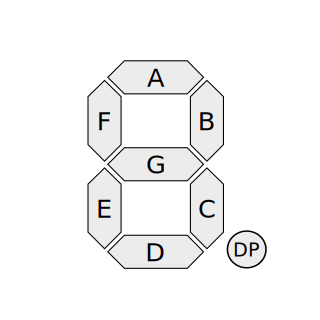
\includegraphics[height=3cm]{pictures/7segdetails.pdf}}
	\caption{Détail et Annotation d'un 7 segment par \href{https://commons.wikimedia.org/wiki/User:H2g2bob}{H2g2bob} - \ccLogo\ccAttribution\ccShareAlike}
\end{figure}

\begin{table}[H]
\centering
\begin{tabular}{|c|c|c|c|c|c|c|c|}
	\hline
		& \multicolumn{7}{c|}{Individual Segments} \\
	\hline
	Display & A & B & C & D & E & F & G \\
	\hline
	0       & 1 & 1 & 1 & 1 & 1 & 1 & 0 \\
	\hline
	1       & 0 & 1 & 1 & 0 & 0 & 0 & 0 \\
	\hline
	2       & 1 & 1 & 0 & 1 & 1 & 0 & 1 \\
	\hline
	3       & 1 & 1 & 1 & 1 & 0 & 0 & 1 \\
	\hline
	4       & 0 & 1 & 1 & 0 & 0 & 1 & 1 \\
	\hline
	5       & 1 & 0 & 1 & 1 & 0 & 1 & 1 \\
	\hline
	6       & 1 & 0 & 1 & 1 & 1 & 1 & 1 \\
	\hline
	7       & 1 & 1 & 1 & 0 & 0 & 0 & 0 \\
	\hline
	8       & 1 & 1 & 1 & 1 & 1 & 1 & 1 \\
	\hline
	9       & 1 & 1 & 1 & 1 & 0 & 1 & 1 \\
	\hline
	A       & 1 & 1 & 1 & 0 & 1 & 1 & 1 \\
	\hline
	B       & 0 & 0 & 1 & 1 & 1 & 1 & 1 \\
	\hline
	C       & 1 & 0 & 0 & 1 & 1 & 1 & 0 \\
	\hline
	D       & 0 & 1 & 1 & 1 & 1 & 0 & 1 \\
	\hline
	E       & 1 & 0 & 0 & 1 & 1 & 1 & 1 \\
	\hline
	F       & 1 & 0 & 0 & 0 & 1 & 1 & 1 \\
	\hline
\end{tabular}
	\caption{Décomposition des caractères hexadécimaux en segments}
\end{table}

\subsection{Mise en place sur logisim}
\paragraph{}
La table de vérité présentée dans la section précèdente peut être utilisée pour obtenir une fonction simplifiée de chaque segment en utilisant les tables de Karnaugh\footnote{\url{https://fr.wikipedia.org/wiki/Table_de_Karnaugh}}. Logisim embarque une fonctionnalité permettant d'effectuer cette analyse de manière simplifiée. Pour celà il est nécessaire de lancer logisim avec l'option -analyze soit dans notre cas :

\begin{lstlisting}[language=bash]
java -jar logisim-evolution.jar -analyze
\end{lstlisting}

\paragraph{}
En utilisant ce paramètre une option apparaît dans le menu "Projet"->"Analyser le circuit". Il est possible dans l'onglet "table" de remplir la table de vérité du circuit. Une fois le tableau complété, cliquer sur "Construire le circuit" générera le circuit correspondant. Ce dernier devrait ressembler à ceci :
\begin{figure}[H]
        \makebox[\textwidth]{\includegraphics[width=4cm]{pictures/sevendecoder.png}}
	\caption{Contenu du composant "Seven segment decoder"}
\end{figure}



\section{Répartition des rôles}
\subsection{Nyan}
\subsubsection{Meow}
\subsubsubsection{Mjau}
MiaouNyanMeowMjau


\section{ALU}

\subsection{Description}

	L'unité arithmétique et logique est l'élèment qui se charge des calculs au sein du processeur. Les ALU les plus basiques ne font que des opérations sur des entiers cependant on trouve des ALU spécialisées. Les calculs sur ces dernières vont des opérations à virgule flottante jusqu'à des calculs plus complexes tels que des racines carrées, des logarithmes, des sinus ou cosinus... Notre ALU n'effectuera que des calculs simples (addition, soustraction, multiplication, décalage) sur des entiers de 32 bits.

	Une ALU comporte deux entrées amenant les données à traiter. Une troisième entrée permet de désigner le calcul à effectuer. En sortie on retrouvera le résultat de l'opération ainsi que des drapeaux. Ces drapeaux représentent une série d'état à la suite d'un calcul : un résultat négatif, un résultat nul, un débordement ou encore une retenue. 

L'entrée \texttt{Shift} indique le nombre de décalage pour les opérations de décalage.


\paragraph{Remarque:} les instructions \texttt{TST}, \texttt{CMP}, \texttt{CMN} n'enregistrent pas le résultat de l'opération. Seuls les drapeaux sont mis à jour.
Pour ces opérations en particulier, il faudra recopier l'entrée \texttt{B} sur la sortie \texttt{S}. Le contrôleur définiera le même registre pour le registre \texttt{Rn} d'opérande B que pour le registre \texttt{Rd} de destination de la sortie S.

\paragraph{Remarque 2:} pour l'instruction \texttt{SBC}, la retenue entrante doit être inversée (voir \textit{\ref{subsubsubsec:SBC}~\nameref{subsubsubsec:SBC}}).

\subsection{Interface}

\subsubsection{Entrées}

\begin{tabular}{|l|r|l|}
\hline
\textbf{Port}		& \textbf{Taille} & \textbf{Description}\\
\hline

\texttt{A}		& \texttt{32} & Première opérande\\
\hline
\texttt{B}		& \texttt{32} & Seconde opérande\\
\hline
\texttt{Shift}		&  \texttt{5} & Nombre de décalage\\
\hline
\texttt{CarryIn}	&  \texttt{1} & Retenu entrente\\
\hline
\texttt{Codop}		&  \texttt{4} & Code opération ALU\\

\hline
\end{tabular}


\subsubsection{Sorties}

\begin{tabular}{|l|r|l|}
\hline 
\textbf{Port} & \textbf{Taille} & \textbf{Description}\\
\hline

\texttt{S}	& \texttt{32} & Registre résultat\\
\hline
\texttt{Flags}	&  \texttt{4} & Registre drapeaux, ordre: \texttt{NZCV}\\

\hline
\end{tabular}


\subsection{Opérations}
\label{subsec:Opcodes}
Ces opérations de l'ALU correspondent exactement aux instructions de la catégorie \textit{Data Processing}. En cas de doute, se référer à \textit{\ref{sec:ISA}~\nameref{sec:ISA}}.

\begin{tabular}{|r|c|l|l|}
\hline
\textbf{Codop}  & \textbf{Opération}	& \textbf{Instructions} & \textbf{Remarque}\\
\hline

$0000$ & \texttt{A and B}			& AND			&\\
\hline
$0001$ & \texttt{A xor B}			& EOR			&\\
\hline
$0010$ & \texttt{B << Shift}			& LSL			& Retenue sortante, voir jeu d'instruction\\
\hline
$0011$ & \texttt{B >> Shift}			& LSR			& Retenue sortante, voir jeu d'instruction\\
\hline
$0100$ & \texttt{B >> Shift (arith)}		& ASR			& Retenue sortante, voir jeu d'instruction\\
\hline
$0101$ & \texttt{A + B + CarryIn}		& ADC			&\\
\hline
$0110$ & \texttt{A – B + CarryIn – 1}		& SBC			& Retenue entrante inversée\\
\hline
$0111$ & \texttt{B >> Shift (rot)}		& ROR			& Retenue sortante, voir jeu d'instruction\\
\hline
$1000$ & \texttt{A and B}			& TST			& Résultat perdu, seuls les drapeaux sont mis à jour\\
\hline
$1001$ & \texttt{0 – A}				& RSB			& Registre Rm utilisé plutôt que Rn\\
\hline
$1010$ & \texttt{A – B}				& CMP			& Résultat perdu, seuls les drapeaux sont mis à jour\\
\hline
$1011$ & \texttt{A + B}				& CMN			& Résultat perdu, seuls les drapeaux sont mis à jour\\
\hline
$1100$ & \texttt{A or B}			& ORR			&\\
\hline
$1101$ & \texttt{A * B}				& MUL			&\\
\hline
$1110$ & \texttt{A and not B}			& BIC			&\\
\hline
$1111$ & \texttt{Not B}				& MVN			&\\
\hline
\end{tabular}

\subsection{Drapeaux}

Ces drapeaux de l'ALU correspondent exactement aux drapeaux de l'architecture ARM. En cas de doute, se référer à \textit{\ref{sec:ISA}~\nameref{sec:ISA}} et \textit{\ref{subsec:Flags}~\nameref{subsec:Flags}} .

\begin{tabular}{|c|l|l|}
\hline
\textbf{Symbole} & \textbf{Nom} & \textbf{Description}\\
\hline

\texttt{N}	& \texttt{Negative}	& Résultat négatif\\
\hline
\texttt{Z}	& \texttt{Zero}		& Résultat nul\\
\hline
\texttt{C}	& \texttt{CarryOut}	& Retenue sortante (dépassement de capacité non-signé)\\
\hline
\texttt{V}	&  \texttt{Overflow}	& Dépassement de capacité signé\\

\hline
\end{tabular}

\section{Banc de registres}

\subsection{Description}

\subsection{Interface}

\subsubsection{Entrées}

\begin{tabular}{|l|r|l|}
\hline
\textbf{Port}		& \textbf{Taille} & \textbf{Description}\\
\hline

\texttt{DataIn}		& \texttt{32} & Données entrantes, à enregistrer dans le registre sélectionné\\
\hline
\texttt{RegDest}	&  \texttt{3} & Sélection du registre de destination des données entrantes\\
\hline
\texttt{Clk}		&  \texttt{1} & Horloge\\
\hline
\texttt{Reset}		&  \texttt{1} & Remise à zéro\\
\hline
\texttt{RegA}		&  \texttt{3} & Sélection du registre A pour les données sortantes\\
\hline
\texttt{RegB}		&  \texttt{3} & Sélection du registre B pour les données sortantes\\

\hline
\end{tabular}


\subsubsection{Sorties}

\begin{tabular}{|l|r|l|}
\hline 
\textbf{Port} & \textbf{Taille} & \textbf{Description}\\
\hline

\texttt{AOut}	& \texttt{32} & Données sortantes du registre sélectionné A\\
\hline
\texttt{BOut}	& \texttt{32} & Données sortantes du registre sélectionné B\\
\hline
\texttt{R0}	& \texttt{32} & Registre interne 0\\
\hline
\texttt{R1}	& \texttt{32} & Registre interne 1\\
\hline
\texttt{R2}	& \texttt{32} & Registre interne 2\\
\hline
\texttt{R3}	& \texttt{32} & Registre interne 3\\
\hline
\texttt{R4}	& \texttt{32} & Registre interne 4\\
\hline
\texttt{R5}	& \texttt{32} & Registre interne 5\\
\hline
\texttt{R6}	& \texttt{32} & Registre interne 6\\
\hline
\texttt{R7}	& \texttt{32} & Registre interne 7\\

\hline
\end{tabular}

Les sorties \texttt{R0-R7} ne seront pas utilisées pour implémenter une quelconque fonctionalité. Elles sont présentes pour aider à visualiser le comportement du processeur.

\subsection{Interaction avec l'ALU}

Après avoir réalisé l'ALU et le banc de registres, l'interaction entre ces composants peut être mise en oeuvre de la manière suivante:

\hspace{14em}
\includegraphics[scale=0.5]{pictures/ALU_Registers.pdf}

Il est ainsi possible de valider leur comportement en enregistrant des données dans le banc de registre (à l'aide des ports \texttt{DataIn} et \texttt{RegDest})
puis en effectuant diverses opération par l'ALU en spécifiant  le \texttt{Codop}.

\section{Contrôleur}

\subsection{Description}
\paragraph{}
Le contrôleur ou unité de contrôle (Control unit en anglais) joue le rôle de chef d'orchestre au sein du processeur. Il est en charge du décodage des instructions. En fonction des informations récupérées au sein de l'instruction et des différents drapeaux, le controleur va agir sur le chemin de données.

\paragraph{}
Il est responsable du choix de la source fournissant les données. La sortie \texttt{Load} selon si elle est à 0 ou à 1 choisira respectivement un chargement depuis l'ALU ou directement depuis la RAM.
Le même méchanisme est utilisé pour choisir la source du nombre de décalage, des immédiats 8 (voir tableau des sorties).

\paragraph{}
Le contrôleur abrite de plus le compteur ordinal et l'incrèmente lorsqu'il traite une instruction.
\subsection{Interface}

\subsubsection{Entrées}

\begin{tabular}{|l|r|l|}
\hline
\textbf{Port}		& \textbf{Taille} & \textbf{Description}\\
\hline

\texttt{Inst}		& \texttt{16} & Instruction à traiter\\
\hline
\texttt{Flags}		&  \texttt{4} & Drapeaux en entrée, ordre \texttt{NZCV}\\
\hline
\texttt{Clk}		&  \texttt{1} & Horloge\\
\hline
\texttt{Reset}		&  \texttt{1} & Remise à Zero\\
\hline


\hline
\end{tabular}


\subsubsection{Sorties}

\begin{tabular}{|l|r|l|}
\hline 
\textbf{Port} & \textbf{Taille} & \textbf{Description}\\
\hline

\hline
\texttt{Carry}		&  \texttt{1} & Retenue sortante (provenant des drapeaux) à destination de l'ALU\\
\hline
\texttt{DP\_Shift}	&  \texttt{1} & Provenance du nombre de décalages: 0 pour registre A, 1 pour Imm5 \\
\hline
\texttt{Imm32\_Enable}	&  \texttt{1} & Provenance de la donnée A: 0 pour registre, 1 pour Imm32\\
\hline
\texttt{Imm5}		&  \texttt{5} & Nombre de décalage pour les instructions de décalage de la catégorie \textit{Shift, add, sub, mov}\\
\hline
\texttt{Imm32}		&  \texttt{8} & Valeur pour les instructions \texttt{MOV}, \texttt{ADD (immediate)} et \texttt{SUB (immediate)}\\
\hline
\texttt{ALU\_Opcode}	&  \texttt{4} & Code opération à destination de l'ALU\\
\hline
\texttt{Rm}		&  \texttt{3} & Séléction du registre pour lecture de l'opérande A\\
\hline
\texttt{Rn}		&  \texttt{3} & Sélection du registre pour lecture de l'opérande B\\
\hline
\texttt{Rd}		&  \texttt{3} & Sélection du registre pour enregistrement du résultat\\
\hline
\texttt{RAM\_Addr}	& \texttt{32} & Adresse mémoire des instructions \textit{Load/Store}\\
\hline
\texttt{Load}		&  \texttt{1} & Provenance des données en entrée du banc de registre\\
\hline
\texttt{Store}		&  \texttt{1} & 1 pour stocker la valeur du registre \texttt{Rm} à l'adress \texttt{RAM\_Address}\\
\hline
\texttt{PC}		&  \texttt{8} & Compteur ordinal: adresse de la prochaine instruction en ROM\\


\hline
\end{tabular}

\subsection{Sous composants}

\subsubsection{Décodeur d'instruction}

\subsubsubsection{Description}

Le bloc \textit{Opcode Decoder} active l'une de ses sorties en fonction de la catégorie d'instruction reconnue, afin d'activer les blocs correspondant du contrôleur.

L'entrée \texttt{Opcode} correspond au code opération pré-extrait de l'instruction, c'est à dire les 6 bits de poids fort de l'instruction.

Les sorties doivent être activées en fonction du code binaire correspondant à chacune d'elle. Voir \textit{\ref{sec:ISA}~\nameref{sec:ISA}}.

\subsubsubsection{Interface}

\textbf{Entrées}\\

\begin{tabular}{|l|r|l|}
\hline
\textbf{Port}	& \textbf{Taille} & \textbf{Description}\\
\hline

\texttt{Opcode}	& \texttt{6} & Code opération à décoder\\

\hline
\end{tabular}

\vspace{1em}
\textbf{Sorties}\\

\begin{tabular}{|l|r|l|}
\hline 
\textbf{Port} & \textbf{Taille} & \textbf{Description}\\
\hline

\texttt{Shift}			&  \texttt{1} & Active le bloc \textit{Shift, add, sub, mov}\\
\hline
\texttt{Data\_Processing}	&  \texttt{1} & Active le bloc \textit{Data Processing}\\
\hline
\texttt{Load\_Store}		&  \texttt{1} & Active le bloc \textit{Load/Store}\\
\hline
\texttt{SP\_Address}		&  \texttt{1} & Active le bloc \textit{SP Address}\\
\hline
\texttt{Branch}			&  \texttt{1} & Active le bloc \textit{Conditional}\\

\hline
\end{tabular}




\subsubsection{Shift, add, sub, mov}

\subsubsubsection{Description}

Le bloc \textit{Shift, add, sub, mov} traite les instructions de calcul de la catégorie \texttt{Shift, add, sub, mov} (voir \textit{\ref{subsubsec:ShiftAddSubMov}~\nameref{subsubsec:ShiftAddSubMov}}).

La sortie \texttt{ALU\_Opcode} devra être définie pour chacune des instructions afin d'exécuter la bonne opération dans l'ALU (voir \textit{\ref{subsec:Opcodes}~\nameref{subsec:Opcodes}}).

Certaines instructions ne mettent pas à jour tous les drapeaux. La sortie \texttt{Flags\_Update\_Mask} doit être définie en conséquence avec le masque dont les bits à 1 correspondent aux drapeaux à mettre à jour.

La sortie \texttt{Carry} force la valeur de la retenue entrante pour l'ALU. Les instructions \texttt{ADD} et \texttt{SUB} n'utilisent pas de retenue entrante.
Elle doit être définie à 0 pour \texttt{ADD} et à 1 pour \texttt{SUB} étant donnée qu'elle est est inversée pour la soustraction dans l'ALU.

La sortie \texttt{Imm32} est utilisée pour communiquer les valeurs des immédiats de \texttt{MOV}, \texttt{ADD} et \texttt{SUB} à l'ALU. Dans ce cas, la sortie \texttt{Imm32\_Enable} doit être définie à 1.
Les immédiats devront être étendus de 3 ou 8 bits vers 32 bits en complétant par des zéros (ce sont des entiers non-signés).

La sortie \texttt{Imm5} est utilisée en tant que valeur du nombre de décalage pour les instructions de décalage \texttt{LSL}, \texttt{LSR} et \texttt{ASR}.

Si l'entrée \texttt{Enable} est à 0, les sorties sont forcées à 0.

\paragraph{Remarque:} l'immédiat pour l'instruction \texttt{MOV} passe par l'ALU pour être enregistré dans le registre de destination.
Pour que la valeur ne soit pas modifiée, on peut l'inverser ici et utiliser l'opération \texttt{RSB} dans l'ALU.

\paragraph{Remarque 2:} pour les opérations de décalage, on préfèrera utiliser le registre \texttt{Rn} à la place de \texttt{Rm} pour rester cohérent avec les instructions de la catégorie \textit{Data Processing}. L'ALU travaillera uniquement sur l'opérande B.

\paragraph{Remarque 3:} quand une instruction ne fait pas usage de certaines sorties, elles doivent être définies à 0.


\subsubsubsection{Interface}

\textbf{Entrées}\\

\begin{tabular}{|l|r|l|}
\hline
\textbf{Port}		& \textbf{Taille} & \textbf{Description}\\
\hline

\texttt{Instruction}	& \texttt{16} & Instruction \textit{Shift, add, sub, mov} à décoder\\
\hline
\texttt{Enable}		&  \texttt{1} & Active le composant. Si 0, les sortie sont forcées à 0\\


\hline
\end{tabular}

\vspace{1em}
\textbf{Sorties}\\

\begin{tabular}{|l|r|l|}
\hline 
\textbf{Port} & \textbf{Taille} & \textbf{Description}\\
\hline

\texttt{ALU\_Opcode}		&  \texttt{4} & Code opération à destination de l'ALU\\
\hline
\texttt{Rm}			&  \texttt{3} & Sélection du registre opérande A\\
\hline
\texttt{Rn}			&  \texttt{3} & Sélection du registre opérande B\\
\hline
\texttt{Rd}			&  \texttt{3} & Sélection du registre résultat\\
\hline
\texttt{Flags\_Update\_Mask}	&  \texttt{4} & Masque de mise à jour des drapeaux à destination du bloc \textit{Flags APSR}\\
\hline
\texttt{Carry}			&  \texttt{1} & Valeur à utiliser en tant que retenue entrante pour l'ALU\\
\hline
\texttt{Imm32\_Enable}		&  \texttt{1} & Indique au processeur d'utiliser la sortie Imm32 à la place du registre Rm\\
\hline
\texttt{Imm5}			&  \texttt{5} & Nombre de décalage à destination de l'ALU\\
\hline
\texttt{Imm32}			& \texttt{32} & Valeur à utiliser en tant qu'opérande A de l'ALU\\

\hline
\end{tabular}








\subsubsection{Data Processing}

\subsubsubsection{Description}

Le bloc \textit{Data Processing} traite les instructions de calcul de la catégorie \texttt{Data Processing} (voir \textit{\ref{subsubsec:DataProc}~\nameref{subsubsec:DataProc}}).

La sortie \texttt{ALU\_Opcode} correspond aux bits 6 à 9, les code opérations de l'ALU ayant été implémenté en conséquence.

Certaines instructions ne mettent pas à jour tous les drapeaux. La sortie \texttt{Flags\_Update\_Mask} doit être définie en conséquence avec le masque dont les bits à 1 correspondent aux drapeaux à mettre à jour.

Si l'entrée \texttt{Enable} est à 0, les sorties sont forcées à 0.

\paragraph{Remarque:} les instructions \texttt{TST}, \texttt{CMP} et \texttt{CMN} ne mettent à jour que les drapeaux et n'enregistrent pas le résultat de l'opération.
Pour celles-ci, le registre \texttt{Rd} sera défini à \texttt{Rn} afin d'être cohérent avec les autres instructions, et que l'ALU puisse copier le contenu de l'opérande B dans le résultat.


\paragraph{Remarque 2:} pour les instructions \texttt{RSB} et \texttt{MUL}, les bits 3 à 5 définissent le registre \texttt{Rn}, contrairement aux autres instructions pour lesquelles ces bits définissent le registre \texttt{Rm}.
Pour simplifier, le registre \texttt{Rm} sera utilisé pour toutes les instructions, en prenant soin de rester cohérent dans l'implémentation de l'ALU.


\subsubsubsection{Interface}

\textbf{Entrées}\\

\begin{tabular}{|l|r|l|}
\hline
\textbf{Port}		& \textbf{Taille} & \textbf{Description}\\
\hline

\texttt{Instruction}	& \texttt{16} & Instruction \textit{Data Processing} à décoder\\
\hline
\texttt{Enable}		&  \texttt{1} & Active le composant. Si 0, les sortie sont forcées à 0\\


\hline
\end{tabular}

\vspace{1em}
\textbf{Sorties}\\

\begin{tabular}{|l|r|l|}
\hline 
\textbf{Port} & \textbf{Taille} & \textbf{Description}\\
\hline

\texttt{ALU\_Opcode}		&  \texttt{4} & Code opération à destination de l'ALU\\
\hline
\texttt{Rm}			&  \texttt{3} & Sélection du registre opérande A\\
\hline
\texttt{Rn}			&  \texttt{3} & Sélection du registre opérande B\\
\hline
\texttt{Rd}			&  \texttt{3} & Sélection du registre résultat\\
\hline
\texttt{Flags\_Update\_Mask}	&  \texttt{4} & Masque de mise à jour des drapeaux à destination du bloc \textit{Flags APSR}\\

\hline
\end{tabular}




\subsubsection{Flags APSR}

\subsubsubsection{Description}


Le bloc \textit{Flags APSR} correspond au 4 bits de poids fort du registre \texttt{Application Program Status Register} de l'architecture ARM. Il conserve les drapeaux générés par la dernière instruction, afin qu'ils soient disponibles pour la prochaine instruction.

L'entrée \texttt{Update\_Mask} permet de réinjecter l'ancien état d'un drapeau si le bit correspondant est à 0. Si le bit est à 1, le drapeau est mis à jour.

\subsubsubsection{Interface}

\textbf{Entrées}\\

\begin{tabular}{|l|r|l|}
\hline
\textbf{Port}		& \textbf{Taille} & \textbf{Description}\\
\hline

\texttt{Flags\_In}	&  \texttt{4} & Nouveaux drapeaux générés par l'instruction courante, ordre \texttt{NZCV}\\
\hline
\texttt{Update\_Mask}	&  \texttt{4} & Masque d'enregistrement des drapeaux, ordre \texttt{NZCV}\\
\hline
\texttt{Clk}		&  \texttt{1} & Horloge\\
\hline
\texttt{Reset}		&  \texttt{1} & Remise à zéro\\


\hline
\end{tabular}

\vspace{1em}
\textbf{Sorties}\\

\begin{tabular}{|l|r|l|}
\hline 
\textbf{Port} & \textbf{Taille} & \textbf{Description}\\
\hline

\texttt{Flags\_Out}	&  \texttt{4} & Drapeaux générés par l'instruction précédente, ordre \texttt{NZCV}\\

\hline
\end{tabular}



\subsubsection{Load/Store}

\subsubsubsection{Description}

Le bloc \textit{Load/Store} traite les instructions de lecture/écriture en mémoire (voir \textit{\ref{subsubsec:LoadStore}~\nameref{subsubsec:LoadStore}}).

La sortie \texttt{RAM\_Addr} correspond à l'adresse mémoire à laquelle effectuer l'opération.
Elle est calculée en fonction de la valeur actuelle du \texttt{Stack\_Pointer} et de l'offset provenant de l'instruction.

La sortie \texttt{Store} indique à la mémoire de stocker la donnée du registre Rm à l'adresse \texttt{RAM\_Addr}. La donnée sera écrite au cycle suivant.

La sortie \texttt{Load} indique au processeur de présenter la donnée à l'adresse \texttt{RAM\_Addr} en entrée du banc de registre (\texttt{DataIn}). La donnée sera disponible au cycle suivant.

La sortie \texttt{PC\_Hold} retarde l'incrémentation du \textit{Program Counter} d'un coup d'horloge. La RAM étant synchrone, elle a besoin d'un cycle pour traiter l'opération de lecture/écriture. La donnée lue n'est donc pas disponible immédiatement, et le processeur ne peut pas commencer à exécuter l'instruction suivante.
La sortie \texttt{Load} devra donc elle aussi être retardée d'un cycle.

Si l'entrée \texttt{Enable} est à 0, les sorties sont forcées à 0.

\paragraph{Astuce:} utiliser une bascule D pour activer \texttt{PC\_Hold} et retarder \texttt{Load}.

\subsubsubsection{Interface}

\textbf{Entrées}\\

\begin{tabular}{|l|r|l|}
\hline
\textbf{Port}		& \textbf{Taille} & \textbf{Description}\\
\hline

\texttt{Instruction}	& \texttt{16} & Instruction de lecture/écriture en mémoire à décoder\\
\hline
\texttt{Enable}		&  \texttt{1} & Active le composant. Si 0, les sortie sont forcées à 0\\
\hline
\texttt{Stack\_Pointer}	& \texttt{32} & Valeur courante du pointeur de pile\\
\hline
\texttt{Clk}		&  \texttt{1} & Horloge\\
\hline
\texttt{Reset}		&  \texttt{1} & Remise à zéro\\


\hline
\end{tabular}

\vspace{1em}
\textbf{Sorties}\\

\begin{tabular}{|l|r|l|}
\hline 
\textbf{Port} & \textbf{Taille} & \textbf{Description}\\
\hline

\texttt{Store}		&  \texttt{1} & Informe d'une opération d'écriture\\
\hline
\texttt{Load}		&  \texttt{1} & Informe d'une opération de lecture\\
\hline
\texttt{PC\_Hold}	&  \texttt{1} & Retarde l'incrémentation du compteur ordinal d'un cycle\\
\hline
\texttt{Rm}		&  \texttt{3} & Registre de provenance de la donnée écrite en mémoire\\
\hline
\texttt{Rd}		&  \texttt{3} & Registre de destination de la donnée lue en mémoire\\
\hline
\texttt{RAM\_Addr}	& \texttt{32} & Adresse mémoire à laquelle effectuer les opérations\\

\hline
\end{tabular}




\subsubsection{SP Address}

\subsubsubsection{Description}

Le bloc \textit{SP Address} traite les instructions de mise à jour du pointeur de pile (voir \textit{\ref{subsubsec:MiscInstr}~\nameref{subsubsec:MiscInstr}}).

La sortie \texttt{New\_Stack\_Pointer} correspond à la nouvelle valeur du pointeur de pile qui sera enregistré dans le \textit{Stack Pointer}.
Elle est calculée en fonction de la valeur actuelle du \texttt{Stack\_Pointer} et de l'opération en provenance de l'instruction (addition ou soustraction d'un immédiat).

Si l'entrée \texttt{Enable} est à 0, la sortie \texttt{Write\_Enable} est forcée à 0.

\subsubsubsection{Interface}

\textbf{Entrées}\\

\begin{tabular}{|l|r|l|}
\hline
\textbf{Port}		& \textbf{Taille} & \textbf{Description}\\
\hline

\texttt{Instruction}	& \texttt{16} & Instruction de mise à jour du pointeur de pile à décoder\\
\hline
\texttt{Enable}		&  \texttt{1} & Active le composant. Si 0, les sortie sont forcées à 0\\
\hline
\texttt{Stack\_Pointer}	& \texttt{32} & Valeur courante du pointeur de pile\\

\hline
\end{tabular}

\vspace{1em}
\textbf{Sorties}\\

\begin{tabular}{|l|r|l|}
\hline 
\textbf{Port} & \textbf{Taille} & \textbf{Description}\\
\hline

\hline
\texttt{Write\_Enable}		&  \texttt{1} & Le registre du pointeur de pile sera mis à jour avec la valeur \texttt{New\_Stack\_Pointer}\\
\hline
\texttt{New\_Stack\_Pointer}	& \texttt{32} & Nouvelle valeur du pointeur de pile\\

\hline
\end{tabular}




\subsubsection{Conditional}

\subsubsubsection{Description}

Le bloc conditionnel traite les instructions de branchement conditionnel (voir \textit{\ref{subsubsubsec:CondBranch}~\nameref{subsubsubsec:CondBranch}}).

Il vérifie la condition à l'aide des drapeaux du registre \textit{Flags APSR}, selon le tableau  \textit{\ref{subsec:CondFlags}~\nameref{subsec:CondFlags}}.
Si la condition est vérifiée, la sortie \texttt{Verified} passe à 1.

La sortie \texttt{Offset} correspond à l'offset qui sera ajouté au \textit{Program Counter}, en provenance de l'instruction.

Si l'entrée \texttt{Enable} est à 0, la sortie \texttt{Verified} est forcée à 0.

\subsubsubsection{Interface}

\textbf{Entrées}\\

\begin{tabular}{|l|r|l|}
\hline
\textbf{Port}		& \textbf{Taille} & \textbf{Description}\\
\hline

\texttt{Instruction}	& \texttt{16} & Instruction du branchement conditionnel à décoder\\
\hline
\texttt{Enable}		&  \texttt{1} & Active le composant. Si 0, les sortie sont forcées à 0\\
\hline
\texttt{N}		&  \texttt{1} & Drapeau négatif\\
\hline
\texttt{Z}		&  \texttt{1} & Drapeau nul\\
\hline
\texttt{C}		&  \texttt{1} & Drapeau retenue\\
\hline
\texttt{V}		&  \texttt{1} & Drapeau dépassement de capacité\\


\hline
\end{tabular}

\vspace{1em}
\textbf{Sorties}\\

\begin{tabular}{|l|r|l|}
\hline 
\textbf{Port} & \textbf{Taille} & \textbf{Description}\\

\hline
\texttt{Verified}	&  \texttt{1} & La condition est vérifiée\\
\hline
\texttt{Offset}		&  \texttt{8} & Offset à appliquer au Program Counter si la condition est vérifiée\\

\hline
\end{tabular}



\subsubsection{Program Counter}

\subsubsubsection{Description}

Le compteur ordinal (\textit{Program Counter}), aussi appelé pointeur d'instruction (\textit{Instruction Pointer}),
est un compteur 8 bits dont la valeur donne l'adresse de la prochaine instruction à exécuter.
Il est déjà implémenté directement dans le contrôleur.

Il s'incrémente automatiquement à chaque coup d'horloge lorsque le signal \texttt{Count} est à l'état haut.
Le signal \texttt{PC\_Hold} sortant du sous-composant \textit{Load/Store} retarde cette incrémentation d'un cycle afin de laisser le temps à la RAM de présenter la donnée sélectionnée sur sa sortie.
En effet, étant synchrone, elle n'agit qu'au coup d'horloge suivant.

Lorsque le signal \texttt{Load} est à l'état haut, le compteur charge la valeur suivante à partir de son entrée au prochain coup d'horloge.
Les instructions de branchement (voir \textit{\ref{subsubsec:Branching}~\nameref{subsubsec:Branching}}) du sous-composant \textit{Conditional} exploitent cette possibilité
afin d'altérer le flot d'exécution du programme en sautant à une certaine adresse.

\paragraph{Remarque:} afin d'être cohérent avec le comportement d'un vrai \texttt{Cortex-M0} et donc rester compatible avec les programmes compilés par \texttt{GCC} ou \texttt{LLVM},
l'offset du branchement est incrémenté de 3.

\subsubsubsection{Interface}

\textbf{Entrées}\\

\begin{tabular}{|l|r|l|}
\hline
\textbf{Port}		& \textbf{Taille} & \textbf{Description}\\
\hline

\texttt{Data}		&  \texttt{8} & Valeur du compteur à définir si \texttt{Load} est à l'état haut\\
\hline
\texttt{Count}		&  \texttt{1} & Active l'incrémentation automatique du compteur\\
\hline
\texttt{UpDown}		&  \texttt{1} & 0: décrémente, 1: incrémente. Forcé à 1.\\
\hline
\texttt{Load}		&  \texttt{1} & Charge la valeur à partir de l'entrée \texttt{Data}\\
\hline
\texttt{Clk}		&  \texttt{1} & Horloge\\
\hline
\texttt{Clear}		&  \texttt{1} & Remise à Zero\\
\hline


\hline
\end{tabular}

\vspace{1em}
\textbf{Sorties}\\

\begin{tabular}{|l|r|l|}
\hline 
\textbf{Port} & \textbf{Taille} & \textbf{Description}\\
\hline

\hline
\texttt{Output}		&  \texttt{8} & Valeur courante du compteur ordinal\\
\hline
\texttt{Carry}		&  \texttt{1} & 1 si le compteur atteint sa valeur maximale. Non utilisé ici.\\

\hline
\end{tabular}


\subsubsection{Stack Pointer}

\subsubsubsection{Description}

Le pointeur de pile (\textit{Stack Pointer}) est un simple registre 32 bits indiquant l'adresse en mémoire du début de la pile.
Il est déjà implémenté directement dans le contrôleur.

Son contenu est modifié par les instructions \texttt{ADD} et \texttt{SUB} 
(voir \textit{\ref{subsubsec:MiscInstr}~\nameref{subsubsec:MiscInstr}}) du sous-composant \textit{SP Address}.

Son contenu est utilisé par les instructions \texttt{LDR} et \texttt{STR} 
(voir \textit{\ref{subsubsec:LoadStore}~\nameref{subsubsec:LoadStore}}) du sous-composant \textit{Load/Store}.

\paragraph{Remarque:} en général dans un programme, on commence par décrémenter (avec \texttt{SUB}) le pointeur de pile de la quantité d'espace mémoire dont on aura besoin. Par la suite, pour les accès mémoire on utilisera \texttt{LDR} et \texttt{STR} avec un offset pour sélectionner le bon emplacement dans la pile. À la fin, on incrémente (avec \texttt{ADD}) le pointeur de pile pour revenir à l'état initial.

On peut dire que la pile grandit vers le bas.

\subsubsubsection{Interface}

\textbf{Entrées}\\

\begin{tabular}{|l|r|l|}
\hline
\textbf{Port}		& \textbf{Taille} & \textbf{Description}\\
\hline

\texttt{Data}		& \texttt{32} & Nouvelle valeur du pointeur de pile\\
\hline
\texttt{Enable}		&  \texttt{1} & Active l'enregistrement de la valeur au prochain coup d'horloge\\
\hline
\texttt{Clk}		&  \texttt{1} & Horloge\\
\hline
\texttt{Reset}		&  \texttt{1} & Remise à Zero\\
\hline


\hline
\end{tabular}

\vspace{1em}
\textbf{Sorties}\\

\begin{tabular}{|l|r|l|}
\hline 
\textbf{Port} & \textbf{Taille} & \textbf{Description}\\
\hline

\hline
\texttt{Output}		& \texttt{32} & Valeur courante du pointeur de pile\\

\hline
\end{tabular}


\documentclass{article}

\usepackage{../parm}
\begin{document}

    \section{Chemin de données}
    \label{sec:DataPath}

    \subsection{Description}

    Il s'agit d'interfacer les différents composants CPU, RAM et ROM afin d'obtenir une machine fonctionelle qui puisse exécuter un programme automatiquement.

    Un bouton \texttt{Reset} contrôle l'entrée \texttt{Reset} du processeur afin de remettre à zéro son état et recommencer l'exécution du programme depuis le début.

    Un bouton \texttt{Clock} contrôle l'entrée \texttt{Clk} du processeur et de la RAM afin de contrôler manuellement l'exécution de chacun des instructions.
    Pour une exécution automatique et pour le déploiement sur FPGA, on utilisera le composant \texttt{Horloge} de Logisim.

    \subsection{CPU}

    \subsubsection{Description}

    Le processeur regroupe le contrôleur, le banc de registres et l'ALU.

    À chaque coup d'horloge, l'instruction est décodée par le contrôleur, le calcul est effectué par l'ALU tandis que le banc de registres lui fournit les données et enregistre le résultat.

    Lors d'une instruction \texttt{LDR}, le signal \texttt{Load} du contrôleur est activé, et la donnée en entrée du banc de registres doit être lue à partir de l'entrée \texttt{RAM\_In} plutôt qu'à partir du résultat de l'ALU.

    Lors d'une instruction \texttt{STR}, le signal \texttt{Store} du contrôleur est activé et est passé à la RAM. Les données en sortie \texttt{RAM\_Out} sont fournies par la sortie \texttt{AOut} du banc de registres.

    Lors d'une instruction de la catégorie \textit{Shift, add, sub, mov}, le signal \texttt{DP\_Shift} du contrôleur est activé et l'immédiat \texttt{Imm5} en sortie du contrôleur est utilisé pour l'entrée \texttt{Shift} de l'ALU.

    Lors d'une instruction de la catégorie \textit{Data Processing}, le signal \texttt{DP\_Shift} du contrôleur est désactivé et les 5 bits de poids faible de la sortie \texttt{AOut} sont utilisés pour l'entrée \texttt{Shift} de l'ALU.

    Lors d'une instruction \texttt{MOV} ou \texttt{ADD} / \texttt{SUB} / \texttt{CMP} avec immédiat, le signal \texttt{Imm32\_Enable} du contrôleur est activé
    et la donnée à l'entrée \texttt{A} de l'ALU doit être lue à partir de la sortie \texttt{Imm32} du contrôleur plutôt qu'à partir de la sortie \texttt{AOut} du banc de registres.

    Les sorties \texttt{Rm}, \texttt{Rn} et \texttt{Rd} du contrôleur se connectent respectivement aux entrées \texttt{RegA}, \texttt{RegB} et \texttt{RegDest} du banc de registres pour sélectionner les registres correspondant.

    Les sorties \texttt{PC} et \texttt{RAM\_Addr} se connectent respectivement aux sorties \texttt{ROM\_Addr} et \texttt{RAM\_Addr} de ce composant CPU pour sélectionner les adresses de la ROM et de la RAM.
    
    Les sorties \texttt{Flags} et \texttt{SP} se connectent aux broches du même nom pour communiquer ces valeurs aux afficheurs de la façade.

    \subsubsection{Interface}

    \subsubsubsection{Entrées}

    \begin{tabular}{|l|r|l|}
        \hline
        \textbf{Port}   & \textbf{Taille} & \textbf{Description}                   \\
        \hline

        \texttt{RAM\_In} & \texttt{32}     & Données chargées à partir de la RAM    \\
        \hline
        \texttt{ROM\_In} & \texttt{16}     & Instruction chargée à partir de la ROM \\
        \hline
        \texttt{Clk}    & \texttt{1}      & Horloge                                \\
        \hline
        \texttt{Reset}  & \texttt{1}      & Remise à Zero                          \\


        \hline
    \end{tabular}

    \subsubsubsection{Sorties}

    \begin{tabular}{|l|r|l|}
        \hline
        \textbf{Port}        & \textbf{Taille}     & \textbf{Description}                                                                       \\
        \hline

        \hline
        \texttt{ROM\_Addr} & \texttt{8}          & Adresse de la prochaine instruction                                                        \\
        \hline
        \texttt{RAM\_Addr} & \texttt{8}          & Adresse de la donnée à lire/écrire en mémoire                                              \\
        \hline
        \texttt{RAM\_Out}  & \texttt{32}         & Donnée à écrire en mémoire                                                                 \\
        \hline
        \texttt{Store}    & \texttt{1}          & Indique à la RAM de sauvegarder la donnée \texttt{RAM\_Out} à l'adresse \texttt{RAM\_Addr} \\
        \hline
        \texttt{R0-R7}    & \texttt{8\times 32} & Sortie des registres utilisées à des fins de débogage et visualisation du comportement     \\
		\texttt{Flags}    & \texttt{4}          & Valeur des drapeaux, issue du contrôleur \\
        \hline
        \texttt{SP}    & \texttt{32}          & Valeur de SP, issue du contrôleur \\

        \hline
    \end{tabular}

    \subsection{RAM}

    \subsubsection{Description}

    La RAM est la mémoire de données dans laquelle le programme vient stocker le contenu d'un registre ou lire une donnée pour remplir un registre.
    Synchrone, elle ne lit ou n'enregistre les données qu'au coup d'horloge suivant.

    Elle est adressée sur 8 bits et contient des données de 32 bits.

    Le signal \texttt{Load} est définit à 1 de manière à toujours obtenir la données à l'adresse \texttt{Address} sur la sortie \texttt{Data}.

    Lorsque le signal \texttt{Store} est activé, les données présentent sur l'entrée \texttt{Input} sont enregistrées dans la RAM à l'adresse \texttt{Address}.

    \paragraph{Remarque:} le jeu d'instructions ARMv7-M adresse la RAM octet par octet (1 adresse = 8 bits de données) tandis que sous Logisim, le composant RAM est adressé mot par mot (1 adresse = 32 bits de données).
    Cela permet de simplifier la gestion de la RAM puisqu'il est possible de charger des données directement dans les registres 32 bits du CPU.

    \paragraph{Remarque 2:} sous Logisim, le paramètre \texttt{Databus implementation} doit être défini à \texttt{Separate databus for read and write}
    et le paramètre \texttt{Trigger} à \texttt{Flanc Montant} afin de pouvoir déployer le composant sur FPGA.

    \subsubsection{Interface}

    \subsubsubsection{Entrées}

    \begin{tabular}{|l|r|l|}
        \hline
        \textbf{Port}   & \textbf{Taille} & \textbf{Description}                               \\
        \hline

        \texttt{Address} & \texttt{8}      & Adresse à laquelle lire/écrire les données         \\
        \hline
        \texttt{Load}   & \texttt{1}      & Lire les données au prochain coup d'horloge        \\
        \hline
        \texttt{Store}  & \texttt{1}      & Enregistrer les données au prochain coup d'horloge \\
        \hline
        \texttt{Clock}  & \texttt{1}      & Horloge                                            \\
        \hline
        \texttt{Input}  & \texttt{32}     & Données à écrire                                   \\


        \hline
    \end{tabular}

    \subsubsubsection{Sorties}

    \begin{tabular}{|l|r|l|}
        \hline
        \textbf{Port}   & \textbf{Taille} & \textbf{Description} \\
        \hline
        \texttt{Data} & \texttt{32}     & Données lues         \\

        \hline
    \end{tabular}

    \subsection{ROM}

    \subsubsection{Description}

    La ROM est la mémoire d'instruction à partir de laquelle les instructions du programme sont lues.
    Elle est accessible en lecture uniquement et est asynchrone.

    Elle est adressée sur 8 bits et contient des données de 16 bits (largeur d'une instruction Thumb).

    Le programme, assemblé par l'assembleur, devra être chargé dans cette ROM

    \subsubsection{Interface}

    \subsubsubsection{Entrées}

    \begin{tabular}{|l|r|l|}
        \hline
        \textbf{Port}   & \textbf{Taille} & \textbf{Description}               \\
        \hline

        \texttt{Address} & \texttt{8}      & Adresse de l'instruction à charger \\

        \hline
    \end{tabular}

    \subsubsubsection{Sorties}

    \begin{tabular}{|l|r|l|}
        \hline
        \textbf{Port}   & \textbf{Taille} & \textbf{Description} \\
        \hline

        \texttt{Data} & \texttt{16}     & Instruction lue      \\

        \hline
    \end{tabular}


%%\subsection{Entrées/Sorties}

\end{document}
\section{Assembleur}

\subsection{Introduction}

	Le code binaire a exécuter est obtenu par l'assemblage d'instructions issus du jeu d'instructions ARMv7 (contre un jeu ARMv6 dans le Cortex-M0 réel).

Le rôle de l'assembleur est de traduire un programme écrit en langage assembleur dans une représentation que le processeur saura interpréter.

Ici, le langage assembleur sera l'UAL (\textit{Unified Assembler Language}) de ARM, restreint aux instructions ARMv7 implémentées.
La représentation des instructions en sortie correspond au codage Thumb des instructions, c'est à dire uniquement sur 16-bits (voir \textit{\ref{sec:ISA}~\nameref{sec:ISA}}).

Le format de sortie aura la particularité d'être un fichier texte lisible par Logisim. Les instructions Thumb devront donc être codées en hexadecimal dans un format décrit ci-après.

\subsection{Syntaxe}
Syntaxe UAL:\\
\texttt{S}: màj des drapeaux\\
\texttt{<c>}: condition\\
\texttt{Rm} registre opérande 1\\
\texttt{Rn}: registre opérande B\\
\texttt{Rd}: registre destination\\
\texttt{<immN>}: immédiat sur \texttt{N} bits\\
\texttt{SP}: registre de pointeur de pile en mémoire\\
\texttt{opcode}: code de l'instruction, peut occuper jusqu'à la taille indiquée\\
\texttt{[]}: argument optionnel\\

Exemple:
Code C :
\lstset{language=C}
\begin{lstlisting}
int main() {
	int a,b,c;
	a = 0;
	b = 1;
	c = a + b;
}
\end{lstlisting}

Code assembleur pour le cortex M0 :
\begin{lstlisting}
	sub	sp, #12
	movs	r0, #0
	str	r0, [sp, #8]
	movs	r1, #1
	str	r1, [sp, #4]
	ldr	r1, [sp, #8]
	ldr	r2, [sp, #4]
	adds	r1, r1, r2
	str	r1, [sp]
	add	sp, #12
\end{lstlisting}

\subsection{Syntaxe Logisim}

Voici un exemple de fichier lisible par Logisim pour remplir le contenu de la ROM:

\begin{lstlisting}
v2.0 raw
b08c 2000 9008 21ff 9104 9000 defe 9800
9904 4288 da08 defe 9800 9908 4081 9108
defe 9800 1c40 9000 def0 b00c
\end{lstlisting}

On observe dont un entête \texttt{v2.0 raw}, toujours présent sur la première ligne.

Sur les lignes suivantes, les instructions sont disposées par groupes de 4 caractères hexadecimaux séparés par des espaces, ce qui représente 32 bits. On a donc deux instructions par groupes. Les retours à la ligne sont optionnels.

\section{Deploiement sur FPGA}

\subsection{Introduction}

Un \textit{FPGA} est un circuit logique programmable. C'est un circuit intégré qui peut être configuré pour effectuer une certaine tâche. La configuration du circuit est souvent décrite dans un langage de description de matériel, par exemple \texttt{VHDL}.

Le but ici n'est pas d'écrire directement du \texttt{VHDL}, mais de le faire générer par Logisim à partir du circuit du processeur.
Il sera donc possible d'observer le comportement du processeur sur du vrai matériel, ici la carte de développement \textit{Altera DE2} avec un FPGA \textit{Cyclone II}, et l'interfacer avec le monde extérieur.

\subsection{Installation de Quartus sur Ubuntu}
\subsubsection{Dépendances}
\noindent Dans Ubuntu 16.04
\vspace{0.2em}
\begin{enumerate}
	\item Installer les paquets suivants:
	\begin{itemize}
		\item \texttt{libc6-i386}
		\item \texttt{libx11-6:i386}
		\item \texttt{libxext6:i386}
	\end{itemize}
	à l'aide de la commande
	\begin{lstlisting}
sudo apt install libc6-i386 libx11-6:i386 libxext6:i386
	\end{lstlisting}

	\item Ajouter le fichier de règles \texttt{51-usbblaster.rules} pour l'accès à l'USB de la carte, disponible à l'adresse \url{https://files.miaounyan.eu/Quartus/}:
	\begin{lstlisting}
sudo cp 51-usbblaster.rules /etc/udev/rules.d/
	\end{lstlisting}
	\item Recharger les règles udev
	\begin{lstlisting}
sudo udevadm control --reload
	\end{lstlisting}
\end{enumerate}

\subsubsection{Installation}
\noindent Dans Ubuntu 16.04
\begin{enumerate}
	\item Télécharger \texttt{QuartusSetupWeb-13.0.1.232.run} et \texttt{cyclone\_web-13.0.232.qdz} à l'adresse: \\
	\url{https://files.miaounyan.eu/Quartus/}
	\item Définir \texttt{QuartusSetupWeb-13.0.1.232.run} comme exécutable:
		\begin{itemize}
			\item À l'aide d'un gestionnaire de fichier graphique
			\begin{enumerate}
				\item Clic droit sur \texttt{QuartusSetupWeb-13.0.1.232.run}
				\item \textit{Proprietés}
				\item Onglet \textit{Permissions}
				\item Cocher \textit{Autoriser l'exécution du fichier comme un programme}
			\end{enumerate}
\vspace{0.2em}
			\item Ou, dans un terminal:
			\begin{lstlisting}
chmod +x QuartusSetupWeb-13.0.1.232.run
			\end{lstlisting}
		\end{itemize}
	\item Double cliquer sur \texttt{QuartusSetupWeb-13.0.1.232.run}
	\item Suivre les étapes d'installation en s'assurant que la prise en charge des FPGA Cyclone est bien sélectionnée, et noter le chemin de destination.
\end{enumerate}

\subsection{Configuration de Logisim}
\noindent Dans Logisim:
\begin{enumerate}
	\item Dans le menu \texttt{FPGA Menu}, sélectionner \texttt{FPGA Commander}
	\item Sélectionner \texttt{ALTERA-DE2} à la ligne \texttt{Choose target board}
	\item Cliquer sur \texttt{Toolpath} et indiquer le dossier correspondant au chemin de destination de l'installation Quartus
	\item Vérifier que les deux premiers boutons indiquent \texttt{VHDL} et \texttt{Download to board}. Dans le cas contraire, cliquer dessus.
\end{enumerate}

\subsection{Déploiement sur la carte}
\begin{enumerate}
        \item Brancher le cable USB à l'ordinateur et à la carte (port de gauche, noté \texttt{BLASTER})
        \item Allumer la carte
\end{enumerate}

\vspace{0.2em}
\noindent Dans VirtualBox
\vspace{0.2em}
\begin{enumerate}
        \item Cliquer sur le menu \texttt{Périphériques}
        \item Dans le sous-menu \texttt{USB}, cocher \texttt{Altera USB-Blaster}
\end{enumerate} 

\noindent Dans Logisim:
\begin{enumerate}
	\item Ouvrir le projet
	\item Dans le menu \texttt{FPGA Menu}, sélectionner \texttt{FPGA Commander}
	\item Sélectionner la fréquence de l'horloge désirée à la ligne \texttt{Choose tick frequency}
	\item Cliquer sur \texttt{Annotate}
	\item Cliquer sur \texttt{Download}
	\item Dans cette boîte de dialogue, cliquer sur \texttt{Load Map} et sélectionner le fichier \texttt{main-ALTERA-DE2-MAP.xml}
	\item Assigner les entrées/sorties restantes en les sélectionnant d'abord dans la colonne de gauche puis en cliquant sur un élément (surligné en rouge) de la carte
	\item Cliquer sur \texttt{Done}
	\item Après avoir patienté quelques instants, confirmer le transfert sur la carte
\end{enumerate}

\section{Jeu d'instructions (Instruction Set Architecture)}
\label{sec:ISA}

Toutes les informations présentes dans cette section proviennent directement du manuel de référence de l'achitecture ARMv7-M (\textit{ARM v7-M Architecture Reference Manual}). Elles ont été traduites et réorganisées pour en faciliter la lecture.
En cas de doute, ou pour en savoir plus, les pages du manuel sont indiquées entre parenthèses.

\subsection{Instructions à implémenter}

\textbf{Binaire:}\\

\begin{tabular}{| c c c c c c c c c c c c c c c c |}
\hline
15 & 14 & 13 & 12 & 11 & 10 & \multicolumn{1}{|c}{9} & 8 & 7 & 6 & 5 & 4 & 3 & 2 & 1 & 0 \\
\hline
\multicolumn{6}{|c}{opcode} & \multicolumn{10}{|c|}{} \\
\hline
\end{tabular}


\subsubsection{Shift, add, sub, mov}
\label{subsubsec:ShiftAddSubMov}

\textbf{Binaire:}\\

\begin{tabular}{| c c c c c c c c c c c c c c c c |}
\hline
15 & 14 & \multicolumn{1}{|c}{13} & 12 & 11 & 10 & 9 & \multicolumn{1}{|c}{8} & 7 & 6 & 5 & 4 & 3 & 2 & 1 & 0 \\
\hline
0 & 0 & \multicolumn{5}{|c}{opcode} & \multicolumn{9}{|c|}{} \\
\hline
\end{tabular}


\subsubsubsection{LSL (immediate): Logical Shift Left (p. 298)}

\textbf{Description: }

Décale le contenu du registre \texttt{Rm} vers la gauche d'un nombre de bits donné par l'immédiat \texttt{imm5}, écrit le résultat dans le registre \texttt{Rd}.\\
Des zéros sont insérés à droite.\\
Les drapeaux suivants sont mis à jour:\\
\texttt{N = 1} si \texttt{résultat < 0}, \texttt{N = 0} sinon.\\                                      
\texttt{Z = 1} si \texttt{résultat = 0}, \texttt{Z = 0} sinon.\\
\texttt{C = Rm<0 - shift>} avec shift le nombre de décalage. Autrement dit, \texttt{C} est égal au dernier bit sortant.\\

\textbf{Assembleur:} T1

\begin{lstlisting}
LSLS <Rd>,<Rm>,#<imm5>
\end{lstlisting}

\textbf{Binaire:}\\

\begin{tabular}{| c c c c c c c c c c c c c c c c |}
\hline
15 & 14 & 13 & \multicolumn{1}{|c}{12} & 11 & \multicolumn{1}{|c}{10} & 9 & 8 & 7 & 6 & \multicolumn{1}{|c}{5} & 4 & 3 & \multicolumn{1}{|c}{2} & 1 & 0 \\
\hline
0 & 0 & 0 & \multicolumn{1}{|c}{0} & 0 & \multicolumn{5}{|c|}{imm5} & \multicolumn{3}{|c|}{Rm} & \multicolumn{3}{|c|}{Rd} \\
\hline
\end{tabular}

\subsubsubsection{LSR (immediate): Logical Shift Right (p. 302)}

\textbf{Description: }

Décale le contenu du registre \texttt{Rm} vers la droite d'un nombre de bits donné par l'immédiat \texttt{imm5}, écrit le résultat dans le registre \texttt{Rd}.\\
Des zéros sont insérés à gauche.\\
Les drapeaux suivants sont mis à jour:\\
\texttt{N = 1} si \texttt{résultat < 0}, \texttt{N = 0} sinon.\\
\texttt{Z = 1} si \texttt{résultat = 0}, \texttt{Z = 0} sinon.\\
\texttt{C = Rm<shift - 1>} avec shift le nombre de décalage. Autrement dit, \texttt{C} est égal au dernier bit sortant.\\

\textbf{Assembleur:} T1

\begin{lstlisting}
LSRS <Rd>,<Rm>,#<imm5>
\end{lstlisting}

\textbf{Binaire:}\\

\begin{tabular}{| c c c c c c c c c c c c c c c c |}
\hline
15 & 14 & 13 & \multicolumn{1}{|c}{12} & 11 & \multicolumn{1}{|c}{10} & 9 & 8 & 7 & 6 & \multicolumn{1}{|c}{5} & 4 & 3 & \multicolumn{1}{|c}{2} & 1 & 0 \\
\hline   
0 & 0 & 0 & \multicolumn{1}{|c}{0} & 1 & \multicolumn{5}{|c|}{imm5} & \multicolumn{3}{|c|}{Rm} & \multicolumn{3}{|c|}{Rd} \\
\hline
\end{tabular}


\subsubsubsection{ASR (immediate): Arithmetic Shift Right (p. 203)}

\textbf{Description: }

Décale le contenu du registre \texttt{Rm} vers la droite d'un nombre de bits donné par l'immédiat \texttt{imm5}, écrit le résultat dans le registre \texttt{Rd}.\\
Le bit de signe de \texttt{Rm} est ré-inséré à gauche.\\
Les drapeaux suivants sont mis à jour:\\
\texttt{N = 1} si \texttt{résultat < 0}, \texttt{N = 0} sinon.\\
\texttt{Z = 1} si \texttt{résultat = 0}, \texttt{Z = 0} sinon.\\
\texttt{C = Rm<shift - 1>} avec shift le nombre de décalage. Autrement dit, \texttt{C} est égal au dernier bit sortant.\\

\textbf{Assembleur:} T1

\begin{lstlisting}
ASRS <Rd>,<Rm>,#<imm5>
\end{lstlisting}

\textbf{Binaire:}\\

\begin{tabular}{| c c c c c c c c c c c c c c c c |}
\hline
15 & 14 & 13 & \multicolumn{1}{|c}{12} & 11 & \multicolumn{1}{|c}{10} & 9 & 8 & 7 & 6 & \multicolumn{1}{|c}{5} & 4 & 3 & \multicolumn{1}{|c}{2} & 1 & 0 \\
\hline   
0 & 0 & 0 & \multicolumn{1}{|c}{1} & 0 & \multicolumn{5}{|c|}{imm5} & \multicolumn{3}{|c|}{Rm} & \multicolumn{3}{|c|}{Rd} \\
\hline
\end{tabular}


\subsubsubsection{ADD (register): Add register (p. 191)}

\textbf{Description: }

Ajoute le contenu du registre \texttt{Rn} au contenu du registre \texttt{Rm}, écrit le résultat dans le registre \texttt{Rd}.\\
Les drapeaux suivants sont mis à jour:\\
\texttt{N = 1} si \texttt{résultat < 0}, \texttt{N = 0} sinon.\\
\texttt{Z = 1} si \texttt{résultat = 0}, \texttt{Z = 0} sinon.\\
\texttt{C = 1} en cas de dépassement de capacité lors d'une opération non signée.\\
\texttt{V = 1} en cas de dépassement de capacité lors d'une opération signée.\\

\textbf{Assembleur:} T1

\begin{lstlisting}
ADDS <Rd>,<Rn>,<Rm>
\end{lstlisting}

\textbf{Binaire:}\\

\begin{tabular}{| c c c c c c c c c c c c c c c c |}
\hline
15 & 14 & 13 & \multicolumn{1}{|c}{12} & 11 & \multicolumn{1}{|c}{10} & \multicolumn{1}{|c}{9} & \multicolumn{1}{|c}{8} & 7 & 6 & \multicolumn{1}{|c}{5} & 4 & 3 & \multicolumn{1}{|c}{2} & 1 & 0 \\
\hline   
0 & 0 & 0 & \multicolumn{1}{|c}{1} & 1 &  \multicolumn{1}{|c}{0} & \multicolumn{1}{|c}{0} & \multicolumn{3}{|c|}{Rm} & \multicolumn{3}{|c|}{Rn} & \multicolumn{3}{|c|}{Rd} \\
\hline
\end{tabular}


\subsubsubsection{SUB (register): Substract register (p. 450)}

\textbf{Description: }
Soustrait le contenu du registre \texttt{Rm} au contenu du registre \texttt{Rn}, écrit le résultat dans le registre \texttt{Rd}.\\
Les drapeaux suivants sont mis à jour:\\
\texttt{N = 1} si \texttt{résultat < 0}, \texttt{N = 0} sinon.\\
\texttt{Z = 1} si \texttt{résultat = 0}, \texttt{Z = 0} sinon.\\
\texttt{C = 1} en cas de dépassement de capacité lors d'une opération non signée.\\    
\texttt{V = 1} en cas de dépassement de capacité lors d'une opération signée.\\

\textbf{Assembleur:} T1

\begin{lstlisting}
SUBS <Rd>,<Rn>,<Rm>
\end{lstlisting}

\textbf{Binaire:}\\

\begin{tabular}{| c c c c c c c c c c c c c c c c |}
\hline
15 & 14 & 13 & \multicolumn{1}{|c}{12} & 11 & \multicolumn{1}{|c}{10} & \multicolumn{1}{|c}{9} & \multicolumn{1}{|c}{8} & 7 & 6 & \multicolumn{1}{|c}{5} & 4 & 3 & \multicolumn{1}{|c}{2} & 1 & 0 \\
\hline   
0 & 0 & 0 & \multicolumn{1}{|c}{1} & 1 &  \multicolumn{1}{|c}{0} & \multicolumn{1}{|c}{1} & \multicolumn{3}{|c|}{Rm} & \multicolumn{3}{|c|}{Rn} & \multicolumn{3}{|c|}{Rd} \\
\hline
\end{tabular}


\subsubsubsection{ADD (immediate): Add 3-bit immediate (p. 189)}

\textbf{Description: }

Ajoute l'immédiat \texttt{Imm3} au contenu du registre \texttt{Rn}, écrit le résultat dans le registre \texttt{Rd}.\\
Les drapeaux suivants sont mis à jour:\\
\texttt{N = 1} si \texttt{résultat < 0}, \texttt{N = 0} sinon.\\
\texttt{Z = 1} si \texttt{résultat = 0}, \texttt{Z = 0} sinon.\\
\texttt{C = 1} en cas de dépassement de capacité lors d'une opération non signée.\\    
\texttt{V = 1} en cas de dépassement de capacité lors d'une opération signée.\\

\textbf{Assembleur:} T1

\begin{lstlisting}
ADDS <Rd>,<Rn>,<#imm3>
\end{lstlisting}

\textbf{Binaire:}\\

\begin{tabular}{| c c c c c c c c c c c c c c c c |}
\hline
15 & 14 & 13 & \multicolumn{1}{|c}{12} & 11 & \multicolumn{1}{|c}{10} & \multicolumn{1}{|c}{9} & \multicolumn{1}{|c}{8} & 7 & 6 & \multicolumn{1}{|c}{5} & 4 & 3 & \multicolumn{1}{|c}{2} & 1 & 0 \\
\hline   
0 & 0 & 0 & \multicolumn{1}{|c}{1} & 1 &  \multicolumn{1}{|c}{1} & \multicolumn{1}{|c}{0} & \multicolumn{3}{|c|}{Imm3} & \multicolumn{3}{|c|}{Rn} & \multicolumn{3}{|c|}{Rd} \\
\hline
\end{tabular}


\subsubsubsection{SUB (immediate): Subtract 3-bit immediate (p. 448)}

\textbf{Description: }

Soustrait l'immédiat \texttt{Imm3} au contenu du registre \texttt{Rn}, écrit le résultat dans le registre \texttt{Rd}.\\
Les drapeaux suivants sont mis à jour:\\
\texttt{N = 1} si \texttt{résultat < 0}, \texttt{N = 0} sinon.\\
\texttt{Z = 1} si \texttt{résultat = 0}, \texttt{Z = 0} sinon.\\
\texttt{C = 1} en cas de dépassement de capacité lors d'une opération non signée.\\    
\texttt{V = 1} en cas de dépassement de capacité lors d'une opération signée.\\

\textbf{Assembleur:} T1

\begin{lstlisting}
SUBS <Rd>,<Rn>,#<imm3>
\end{lstlisting}

\textbf{Binaire:}\\

\begin{tabular}{| c c c c c c c c c c c c c c c c |}
\hline
15 & 14 & 13 & \multicolumn{1}{|c}{12} & 11 & \multicolumn{1}{|c}{10} & \multicolumn{1}{|c}{9} & \multicolumn{1}{|c}{8} & 7 & 6 & \multicolumn{1}{|c}{5} & 4 & 3 & \multicolumn{1}{|c}{2} & 1 & 0 \\
\hline   
0 & 0 & 0 & \multicolumn{1}{|c}{1} & 1 &  \multicolumn{1}{|c}{1} & \multicolumn{1}{|c}{1} & \multicolumn{3}{|c|}{Imm3} & \multicolumn{3}{|c|}{Rn} & \multicolumn{3}{|c|}{Rd} \\
\hline
\end{tabular}


\subsubsubsection{MOV (immediate): Move (p. 312)}

\textbf{Description: }

Écrit l'immédiat \texttt{imm8} dans le registre \texttt{Rd}.\\
Les drapeaux suivants sont mis à jour:\\
\texttt{N = 1} si \texttt{résultat < 0}, \texttt{N = 0} sinon.\\
\texttt{Z = 1} si \texttt{résultat = 0}, \texttt{Z = 0} sinon.\\

\textbf{Assembleur:} T1

\begin{lstlisting}
MOVS <Rd>,#<imm8>
\end{lstlisting}

\textbf{Binaire:}\\

\begin{tabular}{| c c c c c c c c c c c c c c c c |}
\hline
15 & 14 & 13 & \multicolumn{1}{|c}{12} & 11 & \multicolumn{1}{|c}{10} & 9 & 8 & \multicolumn{1}{|c}{7} & 6 & 5 & 4 & 3 & 2 & 1 & 0 \\
\hline
0 & 0 & 1 & \multicolumn{1}{|c}{0} & 0 & \multicolumn{3}{|c|}{Rd} & \multicolumn{8}{|c|}{imm8} \\
\hline
\end{tabular}


\subsubsection{Data processing}
\label{subsubsec:DataProc}

\textbf{Binaire:}\\

\begin{tabular}{| c c c c c c c c c c c c c c c c |}
\hline
15 & 14 & 13 & 12 & 11 & 10 & \multicolumn{1}{|c}{9} & 8 & 7 & 6 & \multicolumn{1}{|c}{5} & 4 & 3 & 2 & 1 & 0 \\
\hline
0 & 1 & 0 & 0 & 0 & 0 & \multicolumn{4}{|c}{opcode} & \multicolumn{6}{|c|}{} \\
\hline
\end{tabular}

\subsubsubsection{AND (register): Bitwise AND (p. 201)}

\textbf{Description: }

Effectue un ET binaire entre le contenu du registre \texttt{Rdn} et le contenu du registre \texttt{Rm}, écrit le résultat dans le registre \texttt{Rdn}.\\
Les drapeaux suivants sont mis à jour:\\
\texttt{N = 1} si \texttt{résultat < 0}, \texttt{N = 0} sinon.\\
\texttt{Z = 1} si \texttt{résultat = 0}, \texttt{Z = 0} sinon.\\
\texttt{C = 0}\\

\textbf{Assembleur:} T1

\begin{lstlisting}
ANDS <Rdn>,<Rm>
\end{lstlisting}

\textbf{Binaire:}\\

\begin{tabular}{| c c c c c c c c c c c c c c c c |}
\hline
15 & 14 & 13 & 12 & 11 & 10 & \multicolumn{1}{|c}{9} & 8 & 7 & 6 & \multicolumn{1}{|c}{5} & 4 & 3 & \multicolumn{1}{|c}{2} & 1 & 0 \\
\hline
0 & 1 & 0 & 0 & 0 & 0 & \multicolumn{1}{|c}{0} & 0 & 0 & 0 & \multicolumn{3}{|c}{Rm} & \multicolumn{3}{|c|}{Rdn} \\
\hline
\end{tabular}


\subsubsubsection{EOR (register): Exclusive OR (p. 239)}

\textbf{Description: }

Effectue un OU exclusif binaire entre le contenu du registre \texttt{Rdn} et le contenu du registre \texttt{Rm}, écrit le résultat dans le registre \texttt{Rdn}.\\
Les drapeaux suivants sont mis à jour:\\
\texttt{N = 1} si \texttt{résultat < 0}, \texttt{N = 0} sinon.\\                                                                  
\texttt{Z = 1} si \texttt{résultat = 0}, \texttt{Z = 0} sinon.\\
\texttt{C = 0}\\

\textbf{Assembleur:} T1

\begin{lstlisting}
EORS <Rdn>,<Rm>
\end{lstlisting}

\textbf{Binaire:}\\

\begin{tabular}{| c c c c c c c c c c c c c c c c |}
\hline
15 & 14 & 13 & 12 & 11 & 10 & \multicolumn{1}{|c}{9} & 8 & 7 & 6 & \multicolumn{1}{|c}{5} & 4 & 3 & \multicolumn{1}{|c}{2} & 1 & 0 \\
\hline
0 & 1 & 0 & 0 & 0 & 0 & \multicolumn{1}{|c}{0} & 0 & 0 & 1 & \multicolumn{3}{|c}{Rm} & \multicolumn{3}{|c|}{Rdn} \\
\hline
\end{tabular}


\subsubsubsection{LSL (register): Logical Shift Left (p. 300)}

\textbf{Description: }

Décale le contenu du registre \texttt{Rdn} vers la gauche d'un nombre de bits donné par l'octet inférieur du registre \texttt{Rm}, écrit le résultat dans le registre \texttt{Rdn}.\\
Des zéros sont insérés à droite.\\
Les drapeaux suivants sont mis à jour:\\
\texttt{N = 1} si \texttt{résultat < 0}, \texttt{N = 0} sinon.\\
\texttt{Z = 1} si \texttt{résultat = 0}, \texttt{Z = 0} sinon.\\
\texttt{C = Rn<0 - shift>} avec shift le nombre de décalage. Autrement dit, \texttt{C} est égal au dernier bit sortant.\\

\textbf{Assembleur:} T1

\begin{lstlisting}
LSLS <Rdn>,<Rm>
\end{lstlisting}

\textbf{Binaire:}\\

\begin{tabular}{| c c c c c c c c c c c c c c c c |}
\hline
15 & 14 & 13 & 12 & 11 & 10 & \multicolumn{1}{|c}{9} & 8 & 7 & 6 & \multicolumn{1}{|c}{5} & 4 & 3 & \multicolumn{1}{|c}{2} & 1 & 0 \\
\hline
0 & 1 & 0 & 0 & 0 & 0 & \multicolumn{1}{|c}{0} & 0 & 1 & 0 & \multicolumn{3}{|c}{Rm} & \multicolumn{3}{|c|}{Rdn} \\
\hline
\end{tabular}



\subsubsubsection{LSR (register): Logical Shift Right (p. 304)}

\textbf{Description: }

Décale le contenu du registre \texttt{Rdn} vers la droite d'un nombre de bits donné par l'octet inférieur du registre \texttt{Rm}, écrit le résultat dans le registre \texttt{Rdn}.\\
Des zéros sont insérés à gauche.\\
Les drapeaux suivants sont mis à jour:\\
\texttt{N = 1} si \texttt{résultat < 0}, \texttt{N = 0} sinon.\\
\texttt{Z = 1} si \texttt{résultat = 0}, \texttt{Z = 0} sinon.\\
\texttt{C = Rn<shift - 1>} avec shift le nombre de décalage. Autrement dit, \texttt{C} est égal au dernier bit sortant.\\

\textbf{Assembleur:} T1

\begin{lstlisting}
LSRS <Rdn>,<Rm>
\end{lstlisting}

\textbf{Binaire:}\\

\begin{tabular}{| c c c c c c c c c c c c c c c c |}
\hline
15 & 14 & 13 & 12 & 11 & 10 & \multicolumn{1}{|c}{9} & 8 & 7 & 6 & \multicolumn{1}{|c}{5} & 4 & 3 & \multicolumn{1}{|c}{2} & 1 & 0 \\
\hline
0 & 1 & 0 & 0 & 0 & 0 & \multicolumn{1}{|c}{0} & 0 & 1 & 1 & \multicolumn{3}{|c}{Rm} & \multicolumn{3}{|c|}{Rdn} \\
\hline
\end{tabular}


\subsubsubsection{ASR (register): Arithmetic Shift Right (p. 205)}

\textbf{Description: }

Décale le contenu du registre \texttt{Rdn} vers la droite d'un nombre de bits donné par l'octet inférieur du registre \texttt{Rm}, écrit le résultat dans le registre \texttt{Rdn}.\\
Le bit de signe de \texttt{Rdn} est ré-inséré à gauche.\\
Les drapeaux suivants sont mis à jour:\\
\texttt{N = 1} si \texttt{résultat < 0}, \texttt{N = 0} sinon.\\
\texttt{Z = 1} si \texttt{résultat = 0}, \texttt{Z = 0} sinon.\\
\texttt{C = Rn<shift - 1>} avec shift le nombre de décalage. Autrement dit, \texttt{C} est égal au dernier bit sortant.\\

\textbf{Assembleur:} T1

\begin{lstlisting}
ASRS <Rdn>,<Rm>
\end{lstlisting}

\textbf{Binaire:}\\

\begin{tabular}{| c c c c c c c c c c c c c c c c |}
\hline
15 & 14 & 13 & 12 & 11 & 10 & \multicolumn{1}{|c}{9} & 8 & 7 & 6 & \multicolumn{1}{|c}{5} & 4 & 3 & \multicolumn{1}{|c}{2} & 1 & 0 \\
\hline
0 & 1 & 0 & 0 & 0 & 0 & \multicolumn{1}{|c}{0} & 1 & 0 & 0 & \multicolumn{3}{|c}{Rm} & \multicolumn{3}{|c|}{Rdn} \\
\hline
\end{tabular}


\subsubsubsection{ADC (register): Add with Carry (p. 187)}

\textbf{Description: }

Ajoute le contenu du registre \texttt{Rm} et le drapeau de retenu au contenu du registre \texttt{Rdn}, écrit le résultat dans le registre \texttt{Rdn}.\\
Les drapeaux suivants sont mis à jour:\\
\texttt{N = 1} si \texttt{résultat < 0}, \texttt{N = 0} sinon.\\
\texttt{Z = 1} si \texttt{résultat = 0}, \texttt{Z = 0} sinon.\\
\texttt{C = 1} en cas de dépassement de capacité lors d'une opération non signée.\\
\texttt{V = 1} en cas de dépassement de capacité lors d'une opération signée.\\

\textbf{Assembleur:} T1

\begin{lstlisting}
ADCS <Rdn>,<Rm>
\end{lstlisting}

\textbf{Binaire:}\\

\begin{tabular}{| c c c c c c c c c c c c c c c c |}
\hline
15 & 14 & 13 & 12 & 11 & 10 & \multicolumn{1}{|c}{9} & 8 & 7 & 6 & \multicolumn{1}{|c}{5} & 4 & 3 & \multicolumn{1}{|c}{2} & 1 & 0 \\
\hline
0 & 1 & 0 & 0 & 0 & 0 & \multicolumn{1}{|c}{0} & 1 & 0 & 1 & \multicolumn{3}{|c}{Rm} & \multicolumn{3}{|c|}{Rdn} \\
\hline
\end{tabular}

\subsubsubsection{SBC (register): Substract with Carry (p. 380)}
\label{subsubsubsec:SBC}

\textbf{Description: }

Soustrait le contenu du registre \texttt{Rm} et le complément du drapeau de retenu au contenu du registre \texttt{Rdn}, écrit le résultat dans le registre \texttt{Rdn}.\\
Les drapeaux suivants sont mis à jour:\\
\texttt{N = 1} si \texttt{résultat < 0}, \texttt{N = 0} sinon.\\
\texttt{Z = 1} si \texttt{résultat = 0}, \texttt{Z = 0} sinon.\\
\texttt{C = 1} en cas de dépassement de capacité lors d'une opération non signée.\\
\texttt{V = 1} en cas de dépassement de capacité lors d'une opération signée.\\

\textbf{Assembleur:} T1

\begin{lstlisting}
SBCS <Rdn>,<Rm>
\end{lstlisting}

\textbf{Binaire:}\\

\begin{tabular}{| c c c c c c c c c c c c c c c c |}
\hline
15 & 14 & 13 & 12 & 11 & 10 & \multicolumn{1}{|c}{9} & 8 & 7 & 6 & \multicolumn{1}{|c}{5} & 4 & 3 & \multicolumn{1}{|c}{2} & 1 & 0 \\
\hline
0 & 1 & 0 & 0 & 0 & 0 & \multicolumn{1}{|c}{0} & 1 & 1 & 0 & \multicolumn{3}{|c}{Rm} & \multicolumn{3}{|c|}{Rdn} \\
\hline
\end{tabular}



\subsubsubsection{ROR (register): Rotate Right (p. 368)}

\textbf{Description: }

Pivote le contenu du registre \texttt{Rdn} vers la droite d'un nombre de bits donné par l'octet inférieur du registre \texttt{Rm}, écrit le résultat dans le registre \texttt{Rdn}.\\
Les bits de \texttt{Rdn} sortant à droite sont ré-insérés à gauche.\\
Les drapeaux suivants sont mis à jour:\\
\texttt{N = 1} si \texttt{résultat < 0}, \texttt{N = 0} sinon.\\
\texttt{Z = 1} si \texttt{résultat = 0}, \texttt{Z = 0} sinon.\\
\texttt{C = résultat<31>}. Autrement dit, \texttt{C} est égal au dernier bit sortant.\\

\textbf{Assembleur:} T1

\begin{lstlisting}
RORS <Rdn>,<Rm>
\end{lstlisting}

\textbf{Binaire:}\\

\begin{tabular}{| c c c c c c c c c c c c c c c c |}
\hline
15 & 14 & 13 & 12 & 11 & 10 & \multicolumn{1}{|c}{9} & 8 & 7 & 6 & \multicolumn{1}{|c}{5} & 4 & 3 & \multicolumn{1}{|c}{2} & 1 & 0 \\
\hline
0 & 1 & 0 & 0 & 0 & 0 & \multicolumn{1}{|c}{0} & 1 & 1 & 1 & \multicolumn{3}{|c}{Rm} & \multicolumn{3}{|c|}{Rdn} \\
\hline
\end{tabular}


\subsubsubsection{TST (register): Set flags on bitwise AND (p. 466)}

\textbf{Description: }

Effectue un ET logique entre le contenu du registre \texttt{Rn} et le contenu du registre \texttt{Rm}, le résultat n'est pas écrit.\\
Les drapeaux suivants sont mis à jour:\\
\texttt{N = 1} si \texttt{résultat < 0}, \texttt{N = 0} sinon.\\
\texttt{Z = 1} si \texttt{résultat = 0}, \texttt{Z = 0} sinon.\\
\texttt{C = 0}\\

\textbf{Assembleur:} T1

\begin{lstlisting}
TST <Rn>,<Rm>
\end{lstlisting}

\textbf{Binaire:}\\

\begin{tabular}{| c c c c c c c c c c c c c c c c |}
\hline
15 & 14 & 13 & 12 & 11 & 10 & \multicolumn{1}{|c}{9} & 8 & 7 & 6 & \multicolumn{1}{|c}{5} & 4 & 3 & \multicolumn{1}{|c}{2} & 1 & 0 \\
\hline
0 & 1 & 0 & 0 & 0 & 0 & \multicolumn{1}{|c}{1} & 0 & 0 & 0 & \multicolumn{3}{|c}{Rm} & \multicolumn{3}{|c|}{Rn} \\
\hline
\end{tabular}



\subsubsubsection{RSB (immediate): Reverse Substract from 0 (p. 372)}

\textbf{Description: }

Soustrait le contenu du registre \texttt{Rn} à l'immédiat 0, écrit le résultat dans le registre \texttt{Rd}.\\
Les drapeaux suivants sont mis à jour:\\
\texttt{N = 1} si \texttt{résultat < 0}, \texttt{N = 0} sinon.\\
\texttt{Z = 1} si \texttt{résultat = 0}, \texttt{Z = 0} sinon.\\
\texttt{C = 0}.\\
\texttt{V = 0}.\\

\textbf{Assembleur:} T1

\begin{lstlisting}
RSBS <Rd>,<Rn>,#0
\end{lstlisting}

\textbf{Binaire:}\\

\begin{tabular}{| c c c c c c c c c c c c c c c c |}
\hline
15 & 14 & 13 & 12 & 11 & 10 & \multicolumn{1}{|c}{9} & 8 & 7 & 6 & \multicolumn{1}{|c}{5} & 4 & 3 & \multicolumn{1}{|c}{2} & 1 & 0 \\
\hline
0 & 1 & 0 & 0 & 0 & 0 & \multicolumn{1}{|c}{1} & 0 & 0 & 1 & \multicolumn{3}{|c}{Rn} & \multicolumn{3}{|c|}{Rd} \\
\hline
\end{tabular}



\subsubsubsection{CMP (register): Compare Registers (p. 231)}

\textbf{Description: }

Soustrait le contenu du registre \texttt{Rm} au contenu du registre \texttt{Rn}, le résultat n'est pas écrit.\\
Les drapeaux suivants sont mis à jour:\\
\texttt{N = 1} si \texttt{résultat < 0}, \texttt{N = 0} sinon.\\
\texttt{Z = 1} si \texttt{résultat = 0}, \texttt{Z = 0} sinon.\\
\texttt{C = 1} en cas de dépassement de capacité lors d'une opération non signée.\\
\texttt{V = 1} en cas de dépassement de capacité lors d'une opération signée.\\

\textbf{Assembleur:} T1

\begin{lstlisting}
CMP <Rn>,<Rm>
\end{lstlisting}

\textbf{Binaire:}\\

\begin{tabular}{| c c c c c c c c c c c c c c c c |}
\hline
15 & 14 & 13 & 12 & 11 & 10 & \multicolumn{1}{|c}{9} & 8 & 7 & 6 & \multicolumn{1}{|c}{5} & 4 & 3 & \multicolumn{1}{|c}{2} & 1 & 0 \\
\hline
0 & 1 & 0 & 0 & 0 & 0 & \multicolumn{1}{|c}{1} & 0 & 1 & 0 & \multicolumn{3}{|c}{Rm} & \multicolumn{3}{|c|}{Rn} \\
\hline
\end{tabular}


\subsubsubsection{CMN (register): Compare Negative (p. 227)}

\textbf{Description: }

Ajoute le contenu du registre \texttt{Rm} au contenu du registre \texttt{Rn}, le résultat n'est pas écrit.\\
Les drapeaux suivants sont mis à jour:\\
\texttt{N = 1} si \texttt{résultat < 0}, \texttt{N = 0} sinon.\\
\texttt{Z = 1} si \texttt{résultat = 0}, \texttt{Z = 0} sinon.\\
\texttt{C = 1} en cas de dépassement de capacité lors d'une opération non signée.\\
\texttt{V = 1} en cas de dépassement de capacité lors d'une opération signée.\\

\textbf{Assembleur:} T1

\begin{lstlisting}
CMN <Rn>,<Rm>
\end{lstlisting}

\textbf{Binaire:}\\

\begin{tabular}{| c c c c c c c c c c c c c c c c |}
\hline
15 & 14 & 13 & 12 & 11 & 10 & \multicolumn{1}{|c}{9} & 8 & 7 & 6 & \multicolumn{1}{|c}{5} & 4 & 3 & \multicolumn{1}{|c}{2} & 1 & 0 \\
\hline
0 & 1 & 0 & 0 & 0 & 0 & \multicolumn{1}{|c}{1} & 0 & 1 & 1 & \multicolumn{3}{|c}{Rm} & \multicolumn{3}{|c|}{Rn} \\
\hline
\end{tabular}


\subsubsubsection{ORR (register): Logical OR (p. 336)}

\textbf{Description: }

Effectue un OU binaire entre le contenu du registre \texttt{Rdn} et le contenu du registre \texttt{Rm}, écrit le résultat dans le registre \texttt{Rdn}.\\
Les drapeaux suivants sont mis à jour:\\
\texttt{N = 1} si \texttt{résultat < 0}, \texttt{N = 0} sinon.\\
\texttt{Z = 1} si \texttt{résultat = 0}, \texttt{Z = 0} sinon.\\
\texttt{C = 0}.\\

\textbf{Assembleur:} T1

\begin{lstlisting}
ORRS <Rdn>,<Rm>
\end{lstlisting}

\textbf{Binaire:}\\

\begin{tabular}{| c c c c c c c c c c c c c c c c |}
\hline
15 & 14 & 13 & 12 & 11 & 10 & \multicolumn{1}{|c}{9} & 8 & 7 & 6 & \multicolumn{1}{|c}{5} & 4 & 3 & \multicolumn{1}{|c}{2} & 1 & 0 \\
\hline
0 & 1 & 0 & 0 & 0 & 0 & \multicolumn{1}{|c}{1} & 1 & 0 & 0 & \multicolumn{3}{|c}{Rm} & \multicolumn{3}{|c|}{Rdn} \\
\hline
\end{tabular}


\subsubsubsection{MUL: Multiply Two Registers (p. 324)}

\textbf{Description: }

Multiplie le contenu du registre \texttt{Rn} avec le contenu du registre \texttt{Rdm}, écrit les 32 bits de poids faible du résultat dans le registre \texttt{Rdm}.\\
Les drapeaux suivants sont mis à jour:\\
\texttt{N = 1} si \texttt{résultat < 0}, \texttt{N = 0} sinon.\\
\texttt{Z = 1} si \texttt{résultat = 0}, \texttt{Z = 0} sinon.\\

\textbf{Assembleur:} T1

\begin{lstlisting}
MULS <Rdm>,<Rn>,<Rdm>
\end{lstlisting}

\textbf{Binaire:}\\

\begin{tabular}{| c c c c c c c c c c c c c c c c |}
\hline
15 & 14 & 13 & 12 & 11 & 10 & \multicolumn{1}{|c}{9} & 8 & 7 & 6 & \multicolumn{1}{|c}{5} & 4 & 3 & \multicolumn{1}{|c}{2} & 1 & 0 \\
\hline
0 & 1 & 0 & 0 & 0 & 0 & \multicolumn{1}{|c}{1} & 1 & 0 & 1 & \multicolumn{3}{|c}{Rn} & \multicolumn{3}{|c|}{Rdm} \\
\hline
\end{tabular}


\subsubsubsection{BIC (register): Bit Clear (p. 213)}

\textbf{Description: }

Effectue un ET binaire entre le contenu du registre \texttt{Rdn} et le contenu du registre \texttt{Rm}, écrit le résultat dans le registre \texttt{Rdn}.\\
Les drapeaux suivants sont mis à jour:\\
\texttt{N = 1} si \texttt{résultat < 0}, \texttt{N = 0} sinon.\\
\texttt{Z = 1} si \texttt{résultat = 0}, \texttt{Z = 0} sinon.\\
\texttt{C = 0}.\\

\textbf{Assembleur:} T1

\begin{lstlisting}
BICS <Rdn>,<Rm>
\end{lstlisting}

\textbf{Binaire:}\\

\begin{tabular}{| c c c c c c c c c c c c c c c c |}
\hline
15 & 14 & 13 & 12 & 11 & 10 & \multicolumn{1}{|c}{9} & 8 & 7 & 6 & \multicolumn{1}{|c}{5} & 4 & 3 & \multicolumn{1}{|c}{2} & 1 & 0 \\
\hline
0 & 1 & 0 & 0 & 0 & 0 & \multicolumn{1}{|c}{1} & 1 & 1 & 0 & \multicolumn{3}{|c}{Rm} & \multicolumn{3}{|c|}{Rdn} \\
\hline
\end{tabular}


\subsubsubsection{MVN (register): Bitwise NOT (p. 328)}

\textbf{Description: }

Effectue un NON binaire sur le contenu du registre \texttt{Rm}, écrit le résultat dans le registre \texttt{Rd}.\\
Les drapeaux suivants sont mis à jour:\\
\texttt{N = 1} si \texttt{résultat < 0}, \texttt{N = 0} sinon.\\
\texttt{Z = 1} si \texttt{résultat = 0}, \texttt{Z = 0} sinon.\\
\texttt{C = 0}.\\

\textbf{Assembleur:} T1

\begin{lstlisting}
MVNS <Rd>,<Rm>
\end{lstlisting}

\textbf{Binaire:}\\

\begin{tabular}{| c c c c c c c c c c c c c c c c |}
\hline
15 & 14 & 13 & 12 & 11 & 10 & \multicolumn{1}{|c}{9} & 8 & 7 & 6 & \multicolumn{1}{|c}{5} & 4 & 3 & \multicolumn{1}{|c}{2} & 1 & 0 \\
\hline
0 & 1 & 0 & 0 & 0 & 0 & \multicolumn{1}{|c}{1} & 1 & 1 & 1 & \multicolumn{3}{|c}{Rm} & \multicolumn{3}{|c|}{Rd} \\
\hline
\end{tabular}


\subsubsection{Load/Store}
\label{subsubsec:LoadStore}

\textbf{Binaire:}\\

\begin{tabular}{| c c c c c c c c c c c c c c c c |}
\hline
15 & 14 & 13 & 12 & \multicolumn{1}{|c}{11} & 10 & 9 & \multicolumn{1}{|c}{8} & 7 & 6 & 5 & 4 & 3 & 2 & 1 & 0 \\
\hline
1 & 0 & 0 & 1 & \multicolumn{3}{|c}{opcode} & \multicolumn{9}{|c|}{} \\
\hline
\end{tabular}

\subsubsubsection{STR (immediate): Store Register (p. 426)}

\textbf{Description: }

Écrit un mot de 32 bits contenu dans le registre \texttt{Rt} à l'adresse mémoire spécifiée.\\
L'adresse mémoire est calculée à partir du contenu du registre \texttt{SP} plus l'immédiat \texttt{imm8}.\\

\textbf{Assembleur:} T2

\begin{lstlisting}
STR <Rt>,[SP,#<imm8>]
\end{lstlisting}

\textbf{Binaire:}\\

\begin{tabular}{| c c c c c c c c c c c c c c c c |}
\hline
15 & 14 & 13 & 12 & \multicolumn{1}{|c}{11} & \multicolumn{1}{|c}{10} & 9 & 8 & \multicolumn{1}{|c}{7} & 6 & 5 & 4 & 3 & 2 & 1 & 0 \\
\hline
1 & 0 & 0 & 1 & \multicolumn{1}{|c}{0} & \multicolumn{3}{|c}{Rt} & \multicolumn{8}{|c|}{imm8} \\
\hline
\end{tabular}


\subsubsubsection{LDR (immediate): Load Register (p. 252)}

\textbf{Description: }

Charge un mot de 32 bits contenu à l'adresse mémoire spécifiée, écrit le résultat dans le registre \texttt{Rt}.\\
L'adresse mémoire est calculée à partir du contenu du registre \texttt{SP} plus l'immédiat \texttt{imm8}.\\

\textbf{Assembleur:} T2

\begin{lstlisting}
LDR <Rt>,[SP{,#<imm8>}]
\end{lstlisting}

\textbf{Binaire:}\\

\begin{tabular}{| c c c c c c c c c c c c c c c c |}
\hline
15 & 14 & 13 & 12 & \multicolumn{1}{|c}{11} & \multicolumn{1}{|c}{10} & 9 & 8 & \multicolumn{1}{|c}{7} & 6 & 5 & 4 & 3 & 2 & 1 & 0 \\
\hline
1 & 0 & 0 & 1 & \multicolumn{1}{|c}{1} & \multicolumn{3}{|c}{Rt} & \multicolumn{8}{|c|}{imm8} \\
\hline
\end{tabular}



\subsubsection{Miscellaneous 16-bit instructions}
\label{subsubsec:MiscInstr}

\textbf{Binaire:}\\

\begin{tabular}{| c c c c c c c c c c c c c c c c |}
\hline
15 & 14 & 13 & 12 & \multicolumn{1}{|c}{11} & 10 & 9 & 8 & 7 & 6 & 5 & \multicolumn{1}{|c}{4} & 3 & 2 & 1 & 0 \\
\hline
1 & 0 & 1 & 1 & \multicolumn{7}{|c}{opcode} & \multicolumn{5}{|c|}{} \\
\hline
\end{tabular}

\subsubsubsection{ADD (SP plus immediate): Add Immediate to SP (p. 193)}

\textbf{Description: }

Ajoute un immédiat à la valeur du registre \texttt{SP}, écrit le résultat dans le registre \texttt{SP}.
Les drapeaux ne sont pas mis à jour.

\textbf{Assembleur:} T2

\begin{lstlisting}
ADD [SP,]SP,#<imm7>
\end{lstlisting}

\textbf{Binaire:}\\

\begin{tabular}{| c c c c c c c c c c c c c c c c |}
\hline
15 & 14 & 13 & 12 & \multicolumn{1}{|c}{11} & 10 & 9 & 8 & \multicolumn{1}{|c}{7} & \multicolumn{1}{|c}{6} & 5 & 4 & 3 & 2 & 1 & 0 \\
\hline
1 & 0 & 1 & 1 & \multicolumn{1}{|c}{0} & 0 & 0 & 0 & \multicolumn{1}{|c}{0} & \multicolumn{7}{|c|}{imm7} \\
\hline
\end{tabular}

\subsubsubsection{SUB (SP minus immediate): Subtract Immediate from SP (p. 452)}

\textbf{Description: }

Soustrait un immédiat à la valeur du registre \texttt{SP}, écrit le résultat dans le registre \texttt{SP}.
Les drapeaux ne sont pas mis à jour.

\textbf{Assembleur:} T1

\begin{lstlisting}
SUB [SP,]SP,#<imm7>
\end{lstlisting}



\textbf{Binaire:}\\

\begin{tabular}{| c c c c c c c c c c c c c c c c |}
\hline
15 & 14 & 13 & 12 & \multicolumn{1}{|c}{11} & 10 & 9 & 8 & \multicolumn{1}{|c}{7} & \multicolumn{1}{|c}{6} & 5 & 4 & 3 & 2 & 1 & 0 \\
\hline
1 & 0 & 1 & 1 & \multicolumn{1}{|c}{0} & 0 & 0 & 0 & \multicolumn{1}{|c}{1} & \multicolumn{7}{|c|}{imm7} \\
\hline
\end{tabular}



\subsubsection{Branch}
\label{subsubsec:Branching}

\textbf{Binaire:}\\

\begin{tabular}{| c c c c c c c c c c c c c c c c |}
\hline
15 & 14 & 13 & 12 & \multicolumn{1}{|c}{11} & 10 & 9 & 8 & \multicolumn{1}{|c}{7} & 6 & 5 & 4 & 3 & 2 & 1 & 0 \\
\hline
1 & 1 & 0 & 1 & \multicolumn{4}{|c}{opcode} & \multicolumn{8}{|c|}{} \\
\hline
\end{tabular}

\subsubsubsection{B: Conditional Branch (p. 207)}
\label{subsubsubsec:CondBranch}

\textbf{Description: }

Continue l'exécution à partir de l'étiquette \texttt{label} si la condition \texttt{<c>} est vérifiée.\\

\textbf{Assembleur:} T1

\begin{lstlisting}
B<c> <label>
\end{lstlisting}

\textbf{Binaire:}\\

\begin{tabular}{| c c c c c c c c c c c c c c c c |}
\hline
15 & 14 & 13 & 12 & \multicolumn{1}{|c}{11} & 10 & 9 & 8 & \multicolumn{1}{|c}{7} & 6 & 5 & 4 & 3 & 2 & 1 & 0 \\
\hline
1 & 1 & 0 & 1 & \multicolumn{4}{|c}{cond} & \multicolumn{8}{|c|}{imm8} \\
\hline
\end{tabular}








\subsection{Conditions (p. 176)}
\label{subsec:CondFlags}

\begin{tabular}{| c | c | c | c |}
\hline
\textbf{code} & \textbf{symbole} & \textbf{signification} & \textbf{drapeaux}\\
\hline
0000 & EQ & égalité & Z == 1\\
\hline
0001 & NE & différence & Z == 0\\
\hline
0010 & CS & retenue & C == 1\\
\hline
0011 & CC & pas de retenue & C == 0\\
\hline
0100 & MI & négatif & N == 1\\
\hline
0101 & PL & positif ou nul & N == 0\\
\hline
0110 & VS & dépassement de capacité & V == 1\\
\hline
0111 & VC & pas de dépassement de capacité & V == 0\\
\hline
1000 & HI & supérieur (non signé) & C == 1 et Z == 0\\
\hline
1001 & LS & inférieur ou égal (non signé) & C == 0 et Z == 1\\
\hline
1010 & GE & supérieur ou égal (signé) & N == V\\
\hline
1011 & LT & inférieur (signé) & N != V\\
\hline
1100 & GT & supérieur (signé) & Z == 0 et N == V\\
\hline
1101 & LE & inférieur ou égal (signé) & Z == 1 ou Z != V\\
\hline
1110 & aucun ou AL & toujours vrai & \\
\hline
\end{tabular}


\subsection{Drapeaux (p. 31)}
\label{subsec:Flags}

\begin{itemize}
	\item \texttt{N}: résultat négatif, égal au bit de poids fort du résultat
	\item \texttt{Z}: résultat nul, égal à 1 si le résultat est 0
	\item \texttt{C}: retenue
	\item \texttt{V}: dépassement de capacité
\end{itemize}



\documentclass{article}

\usepackage{../parm}
\begin{document}

    \section{Pour aller plus loin}

    \subsection{Compilation de code C}
    Avec le jeu d'instructions de ce processeur, il est possible d'exécuter du code C compilé par \texttt{Clang}.
    Il doit cependant rester relativement simple avec une structure bien précise.

    En particulier, on évitera:
    \begin{itemize}
        \item Les appels de fonctions (\texttt{LR}, \texttt{PUSH}, \texttt{POP} non implémentés)
        \item Les variables globales et \texttt{static} (adressage uniquement sur la pile)
        \item Les adressages indirects (donc l'utilisation de tableaux ou de chaînes)
    \end{itemize}

    On s'assurera donc:
    \begin{itemize}
        \item D'écrire tout le code dans la fonction \texttt{void run()}
        \item De déclarer toutes les variables dans le corps de cette dernière
    \end{itemize}
    
    Voici le code de démarrage pour un programme C dans le cadre du projet :
    \lstset{
        basicstyle=\ttfamily,
        keywordstyle=\color[rgb]{0,0,1},
        commentstyle=\color[rgb]{0.133,0.545,0.133},
        stringstyle=\color[rgb]{0.627,0.126,0.941},
        frame=single,
        tabsize=4,
        columns=fixed,
        breaklines=true,
        xleftmargin=0pt,
        postbreak=\mbox{\textcolor{red}{$\hookrightarrow$}\space},
    }
     \begin{lstlisting}[language=C]
#include <parm.h>

void run()
{
	BEGIN();
	// code ici	
	END();
}
    \end{lstlisting}
    
    On utilise ici une fonction s'appelant \texttt{run} et non pas \texttt{main} car les compilateurs C émettent un warning lorsque la fonction \texttt{main()} ne se termine pas (par exemple, si elle contient une boucle infinie). Or, c'est ici un cas souhaité, et appeler la fonction autrement évite ce warning.
    
    Les appels \texttt{BEGIN} et \texttt{END} sont des macros servant à allouer l'espace mémoire nécessaire pour gérer les périphériques d'entrée/sortie. Il faut systématiquement les écrire dans vos programmes en début et en fin de fonction, sans quoi vous ne pourrez pas utiliser la RAM et ne pourrez donc pas utiliser de variables.

    La commande à utiliser est la suivante (écrivez la, si vous la copiez depuis le PDF les caractères ne seront pas bons) :
    \begin{lstlisting}
clang -S -target arm-none-eabi -mcpu=cortex-m0 -O0 -mthumb -nostdlib -I./include main.c
    \end{lstlisting}
    avec \texttt{main.c} le fichier source C. Veillez à être dans le dossier code\_c en lançant cette commande.

    Cela crééra un fichier de sortie \texttt{main.s} contenant les instructions assembleur, entourées de directives spéciales qui ne nous intéressent pas ici.

    \paragraph{Remarque 2:} depuis la version 9 de \texttt{Clang}, l'addressage mémoire est réalisé différemment en utilisant des instructions \texttt{add <Rd>,SP,\#<imm8>} et \texttt{ldr <Rt>,<Rn>,\#<imm5>} qui ne sont pas prises en charge par l'implémentation.
    Il faut donc s'assurer d'utiliser une version 4 à 8 de \texttt{Clang} (paquet \texttt{clang-8} sous Ubuntu).

    Le code assembleur devra être passé à l'assembleur écrit dans le cadre du projet pour générer le fichier lisible par Logisim et pouvoir l'importer dans la ROM.
    
    \subsection{Périphériques d'entrée/sortie mappés en mémoire}
    
    Actuellement, notre processeur ne peut interagir avec l'utilisateur que de façon très primitive :
    \begin{itemize}
	    \item En écrivant une valeur dans un registre
	    \item En lisant ou écrivant une valeur dans la RAM
    \end{itemize}
    
    Dans les deux cas, cela limite à des valeurs numériques, et cela implique de prévoir à l'avance, par convention, dans quel registre ou case mémoire lire ou écrire.
    
    Dans la réalité, vous lisez ce document sur un ordinateur avec lequel vous interagissez via des périphériques d'entrée/sortie : un clavier, une souris, un écran, etc.
    
    Deux méthodes sont principalement utilisées pour gérer de tels périphériques :
    
    \bgroup
    \def\arraystretch{1.5}%  1 is the default, change whatever you need
    \begin{tabularx}{\textwidth}{|X|X|}
    	\hline
    	Entrées/sorties mappées en mémoire (MMIO) & Entrées/sorties mappées en ports (PMIO) \\
    	\hline
    	L'espace mémoire de l'ordinateur contient des sections correspondant non pas à une vraie mémoire, mais à des registres partagés avec des périphériques & Chaque périphérique possède un ou plusieurs "ports" qui lui sont associés, chacun ayant un numéro correspondant, et le processeur possède des instructions spécifiques permettant de lire ou d'écrire dans ces ports \\
    	\hline
    	Utilise les instructions de gestion de RAM & Utilise des instructions spécifiques (ex: \texttt{in} et \texttt{out} en x86 \\
    	\hline
    	Game Boy, [S]NES, Commodore 64, anciens périphériques PC & Compatibles PC modernes (PCs, Macs, smartphones, ...) \\
    	\hline
    \end{tabularx}
    \egroup
    
    De nos jours, c'est l'approche MMIO qui est généralement préférée. L'approche PMIO était très pertinente à l'époque où la mémoire physique était limitée, et où "perdre" une partie de l'espace mémoire en échange de périphériques était trop coûteux. De nos jours, les bus d'adresse de moins de 16 bits se font rares excepté sur les microcontrôleurs, et le PMIO n'est plus utilisé que dans certains cas pour des raisons de compatibilité (ex: port série ou parallèle sur PC).
    
    Le processeur PARM possède une RAM de 256 mots de 32 bits et un bus d'adresse sur 9 bits. Son espace mémoire est disposé de la manière suivante :
    
    \newcommand{\memsection}[4]{
		\bytefieldsetup{bitheight=#3\baselineskip}	% define the height of the memsection
		\bitbox[]{8}{
			\texttt{0x\uppercase{#1}}	 % print end address
			\\ \vspace{#3\baselineskip} \vspace{-2\baselineskip} \vspace{-#3pt} % do some spacing
			\texttt{0x\uppercase{#2}} % print start address
		}
		\bitbox{16}{#4} % print box with caption
	}
	
	\begin{bytefield}{24}
	\begin{rightwordgroup}{mémoire virtuelle}
		\memsection{1ff}{110}{3}{-- inutilisé --}\\
		\memsection{10f}{100}{4}{Ports I/O}
	\end{rightwordgroup}\\
	\begin{rightwordgroup}{mémoire physique}
		\memsection{0ff}{000}{4}{Pile}
	\end{rightwordgroup}\\
\end{bytefield}

	Les 256 premiers mots (adresses $[0;256[$) correspondent à la mémoire RAM physique, tandis que les 256 suivants sont "virtuels", ils sont gérés par le contrôleur MMIO présent en bas du circuit, qui se charge de déléguer aux différents périphériques. Ici, 16 emplacements sont alloués, donc les adresses $[256;271[$ correspondent à des périphériques et les adresses $[271;512[$ ne sont "branchées" à rien.
	
	La documentation des différents périphériques est disponible dans le fichier \texttt{include/parm.h}.
	
	\subsubsection{Exemple : DIP switch}
	
	Un composant d'entrée très courant est le DIP switch. Il s'agit d'un petit bloc comportant une série de $n$ interrupteurs, encodant un nombre sur $n$ bits. Voici à quoi ça ressemble :
	
	\begin{figure}[t]
        \begin{center}
            \includegraphics[width=250pt]{pictures/dip.png}
            \caption{\label{fig_dip_switch}DIP switch}
        \end{center}
    \end{figure}
    
    Notre processeur est relié à trois switches de ce genre, sur les entrées 3, 4 et 5 (adresses 259, 260 et 261). Du point de vue d'un programme, lire depuis les DIP switches revient à lire depuis une variable qui serait stockée à ces emplacements, c'est entièrement transparent.
    
    \subsubsection{Exemple : Terminal}
    
    La manière la plus simple d'afficher du texte est via un terminal. Nommé d'après les terminaux physiques qui équipaient les mini-ordinateurs des années 1970, son fonctionnement est simple : quand il reçoit un caractère, il l'affiche. Certains caractères ont un effet particulier :
    \begin{itemize}
    	\item \texttt{\textbackslash n} (newline) effectue un retour à la ligne
    	\item \texttt{\textbackslash b} (backspace) efface le dernier caractère saisi
    	\item \texttt{\textbackslash f} (form-feed) efface l'écran
    \end{itemize}
    Ainsi, ça évite d'avoir des entrées spécifiques pour toutes ces actions.
    
    En pratique, le terminal de Logisim possède plusieurs entrées : l'horloge, le caractère, la mise à jour et la réinitialisation. Cette dernière n'est utilisée que quand on appuie sur le bouton "Reset" du processeur.
    
    À chaque front montant d'horloge, si la broche "mise à jour" est haute, alors le caractère est affiché.
    
    Une seule sortie est fournie aux programmes : caractère. Sa valeur est reliée à l'entrée "caractère" de l'écran, et dès qu'une écriture est faite dans cette sortie, l'entrée "mise à jour" est passée à 1.
    

\end{document}


\end{document}
